\documentclass{beamer}
\usetheme{Madrid}
\usepackage{amsmath}
\usepackage{amssymb}
\usepackage{graphicx}
\usepackage{physics}
\usepackage{tikz}
\usepackage{simpler-wick}
\usepackage{cancel}
\usepackage{geometry}
\usepackage{algorithm}
\usepackage{algorithmic}
\usepackage[numbers]{natbib}
\bibliographystyle{plainnat}  % or another style like 'apsrev4-2'
\usepackage{hyperref}
\usepackage{bm}
\usepackage{xcolor}
\usepackage{listings}
\newcommand{\red}[1]{\textcolor{red}{#1}}
\newcommand{\green}[1]{\textcolor{green}{#1}}

\title{Slides for Patryk's Notes}
\author{Patryk Kozlowski}
\date{\today}

\hypersetup{
    colorlinks=true,    % false: boxed links; true: colored links
    linkcolor=blue,     % color of internal links
    urlcolor=cyan       % color of external links
}
\setbeamertemplate{section in toc}[sections numbered]

% Automatically create section title slides
\AtBeginSection[]{
  \begin{frame}
  \frametitle{Outline}
  \tableofcontents[currentsection]
  \end{frame}
}

% Alternative: Simple section title slide
% \AtBeginSection[]{
%   \begin{frame}
%   \centering
%   \LARGE \insertsectionhead
%   \end{frame}
% }

\begin{document}

\begin{frame}
    \titlepage
\end{frame}
\begin{frame}
  \frametitle{Outline}
  \tableofcontents
\end{frame}
% \section{SRG-MP2 Update}
\begin{frame}
\frametitle{Derivation starting with the electron-boson Hamiltonian}
The core hole approximation allows us to write
\begin{align}
\hat{c}_p^\dagger \ket{N} &\equiv \hat{c}_p^\dagger \Bigl( |N_F\rangle \otimes |0_B\rangle \Bigr) \approx \hat{c}_p^\dagger \Bigl( |\Phi_0^N\rangle \otimes |0_B\rangle \Bigr)
\label{eq:core_hole_approx_1}\\
& = |\Phi_0^{N-1}\rangle \otimes |0_B\rangle
% & \approx |\Phi_0^{N-1}\rangle \otimes |0_B\rangle \label{eq:core_hole_approx_2} \\
\equiv \ket{\Psi_p}
\end{align}
so with $
    \hat{H}_{\text{eB}} = \underbrace{\epsilon_{p} + \sum_{\nu} \Omega_{\nu} \hat{b}_\nu^\dagger \hat{b}_\nu}_{\hat{H}_0} + \underbrace{\sum_{\nu} W_{p\nu} \left( \hat{b}_\nu^\dagger + \hat{b}_\nu \right)}_{\hat{V}}$
, we get
\begin{align}
G_{pp}^R(t) &= -i \theta(t) \bra{N} \hat{c}_p e^{-i\hat{H} t} \hat{c}_p^\dagger \ket{N} \\
%  &\approx -i \theta(t) \bra{\Psi_p} e^{-i\hat{H}_{\text{eB}} t} \ket{\Psi_p} \\
% &= -i \theta(t) \bra{\Psi_p} e^{-i\left( \hat{H}_0 + \hat{V} \right) t} \ket{\Psi_p} \\
% &\approx -i \theta(t) \bra{\Psi_p} e^{-i\hat{H}_0 t} \mathcal{T} \exp \left( -i \int_0^t dt' e^{i\hat{H}_0 t'} \hat{V} e^{-i\hat{H}_0 t'} \right) \ket{\Psi_p} \\
&\approx -i \theta(t) e^{-i\epsilon_p t} {\bra{\Psi_p}  \mathcal{T} \exp \left( -i \int_0^t dt' V_I(t') \right) \ket{\Psi_p}} \\
&=
-i\,\theta(t)\,e^{-i\epsilon_p t} [1-\sum_\nu |W_{p\nu}|^2\left(\frac{t}{i\Omega_\nu}+\frac{1-e^{-i\Omega_\nu t}}{\Omega_\nu^2}\right) + O(W^4)]
\end{align}
and we identify $C_2(t) = -\sum_\nu |W_{p\nu}|^2\left(\frac{t}{i\Omega_\nu}+\frac{1-e^{-i\Omega_\nu t}}{\Omega_\nu^2}\right)$.
\end{frame}
\begin{frame}
\frametitle{Why this is compatible with SRG-MP2}
The Landau form that I have been using is
\begin{equation}
C(t) = \int d\omega \frac{\beta(\omega)}{\omega^2} \left( e^{-i\omega t} + i\omega t - 1 \right)
\end{equation}
where $\beta(\omega) = -\frac{1}{\pi} \text{Im} \Sigma_{pp}^{(2)}(\omega + \epsilon_p)$. $\Sigma^2$ has 2p1h poles at
 \begin{equation} \epsilon_{pi}^{ab} = \epsilon_a + \epsilon_b - \epsilon_i\end{equation} So $\Sigma^2$ is a linear combination of delta functions located at $\epsilon_{pi}^{ab}$. The QBA tells us that these can be thought of as bosonic frequencies.


\end{frame}
\begin{frame}
\frametitle{Technical issues with SRG-MP2}
\begin{align}
    F_{pq}^{(2)}(s)  &= \frac{1}{2}\sum_{ija}\frac{\Delta^{pa}_{ij} + \Delta^{qa}_{ij}}{\left(\Delta^{pa}_{ij}\right)^2+\left(\Delta^{qa}_{ij}\right)^2} \bra{pa}\ket{ij}\bra{ij}\ket{qa}
    \nonumber \\
    &\times\left[1-e^{-\left[\left(\Delta^{pa}_{ij}\right)^2+\left(\Delta^{qa}_{ij}\right)^2\right]s}\right] \nonumber \\
    &+ \frac{1}{2}\sum_{abi}\frac{\Delta^{pi}_{ab} + \Delta^{qi}_{ab}}{\left(\Delta^{pi}_{ab}\right)^2+\left(\Delta^{qi}_{ab}\right)^2} \bra{pi}\ket{ab}\bra{ab}\ket{qi}
    \nonumber \\
    &\times\left[1-e^{-\left[\left(\Delta^{pi}_{ab}\right)^2+\left(\Delta^{qi}_{ab}\right)^2\right]s}\right]\label{eq:qsGF2SE}.
\end{align}
\begin{itemize}
    \item $\downarrow s \to \uparrow reg. \downarrow \Delta HF; \uparrow s \to \downarrow reg. \uparrow \Delta HF$
    \item How to do self-consistency numerically with fixed pt. and/or  DIIS?
\end{itemize}
\end{frame}
% % \section{What to do about the spectral function discrepancy?}
% \begin{frame}
% \frametitle{HF IPs are derived analytically}
% I got
% \begin{align}
% \epsilon_{ p}^\sigma & = \frac{|\vec{G}_p|^2}{2} -\frac{1}{\Omega} \sum_{i\in occ} \left(\frac{4 \pi}{\left|\vec{G}_p-\vec{G}_i\right|^2} \left(1-\delta_{\vec{G}_p,\vec{G}_i}\right) - \Omega v_{\mathrm{M}}\delta_{\vec{G}_p,\vec{G}_i}\right) \\
% & = \frac{|\vec{G}_p|^2}{2} -\frac{1}{\Omega} \sum_{i\in occ} \frac{4 \pi }{\left|\vec{G}_p-\vec{G}_i\right|^2} \left(1-\delta_{\vec{G}_p,\vec{G}_i}\right) + v_{\mathrm{M}}n^\sigma_{p}
% \end{align}
% This corresponds to taking what you reported but shifting it by $\xi/2$.
% \end{frame}
\section{PT2 variants}
% \begin{frame}
% \frametitle{Review of what I do with the PT2+C spectral functions}
% I presented two varieties of cumulants. The Landau form is
% \begin{align}
%     C_{pp}(t) &\equiv i \int \frac{d\omega}{2\pi} \frac{ \Sigma_{pp}\left(\omega+E_p\right)}{(\omega + i \eta)^2} e^{-i \omega t}
% \label{eq:Cpp_0_updated}
% \end{align}
% and the time domain Green's function in the cumulant ansatz is
% \begin{equation}
%     G_{pp}(t) = \underbrace{-i \Theta(t) e^{-t(i E_p +\eta)}}_{\bm{G}_0} e^{C_{pp}(t)}
% \label{eq:Gpp_time_updated}
% \end{equation}
% In '$G_0$ via HF', $E_p\equiv \epsilon_p^{HF},\{\epsilon_p^{HF}\}\rightarrow\Sigma _{pp}(\omega)$, while in '$G_0$ via SRG', $E_p\equiv \epsilon_p^{SRG-MP2},\{\epsilon_p^{SRG-MP2}\}\rightarrow \Sigma _{pp}(\omega)$. I understand this through
% \begin{equation}
%     \bm{G}(\omega ) = \bm{G}_0(\omega ) + \bm{G}_0(\omega ) \bm{\Sigma}(\omega ) \bm{G}(\omega )
% \end{equation}
% so in \ref{eq:Cpp_0_updated} and \ref{eq:Gpp_time_updated}, the former approach sets $\bm{G}_0\equiv \bm{G}_{HF}$ and the latter sets $\bm{G}_0\equiv \bm{G}_{SRG-MP2}$. \emph{Loos found that for small molecules, SRG-GW+C can be worse than $G_0W_0$+C.}
% \end{frame}
% \begin{frame}
% \frametitle{How SRG-MP2 comes about}
% Derivation can be done, but the final expression is most relevant:
% \begin{align}
%     F_{pq}^{(2)}(s)  &= \frac{1}{2}\sum_{ija}\frac{\Delta^{pa}_{ij} + \Delta^{qa}_{ij}}{\left(\Delta^{pa}_{ij}\right)^2+\left(\Delta^{qa}_{ij}\right)^2} \bra{pa}\ket{ij}\bra{ij}\ket{qa}
%     \nonumber \\
%     &\times\left[1-e^{-\left[\left(\Delta^{pa}_{ij}\right)^2+\left(\Delta^{qa}_{ij}\right)^2\right]s}\right] \nonumber \\
%     &+ \frac{1}{2}\sum_{abi}\frac{\Delta^{pi}_{ab} + \Delta^{qi}_{ab}}{\left(\Delta^{pi}_{ab}\right)^2+\left(\Delta^{qi}_{ab}\right)^2} \bra{pi}\ket{ab}\bra{ab}\ket{qi}
%     \nonumber \\
%     &\times\left[1-e^{-\left[\left(\Delta^{pi}_{ab}\right)^2+\left(\Delta^{qi}_{ab}\right)^2\right]s}\right]\label{eq:qsGF2SE}.
% \end{align}
% The idea is to add this to your HF Fock matrix and iterate to self-consistency. Tolle found that it is optimal to choose $s=1e3$ in his IP/EA tests, so that's what I use.
% \end{frame}
\begin{frame}
\frametitle{Nooijen's approach}
MP2 tells us that we have to diagonalize:
\begin{align}
A_{p q}^{\text {MP2 }}(\omega)
= & \epsilon_{p} \delta_{p q}+\frac{1}{2} \sum_{l, c, d} \frac{V_{p l[c d]} V_{c d[q l]}}{\omega+\epsilon_{l}-\epsilon_{c}-\epsilon_{d}}
-\frac{1}{2} \sum_{k, l, d} \frac{V_{p d[k l]} V_{k l[q d]}}{\epsilon_{k}+\epsilon_{l}-\epsilon_{d}-\omega}
\end{align}
Nooijen starts with CCSD-GF, but then approximates CC amplitudes with MBPT(2) analogues as
\begin{align*}
& t_{i}^{a}=0 \\
& t_{i j}^{a b}=\frac{V_{a b i j}}{\epsilon_{i}+\epsilon_{j}-\epsilon_{a}-\epsilon_{b}}
\end{align*}
They call this MBPT(2)-GF and it leads to $A^{\mathrm{MBPT(2)}}(\omega)$. The paper is not about this theory though, but rather they use it as a starting point for further approximations that reduce cost.
\end{frame}
\begin{frame}
\frametitle{Starting point for DSO-GF}
They first replace the most demanding 2h1p block of $A^{\mathrm{MBPT(2)}}(\omega)$ by a diagonal form, but this is not size-consistent. But it is when the diagonal is approximated with a MP partitioning as

\begin{equation*}
{ }^{\mathrm{DSO}} D_{i j}^{b}=-\epsilon_{i}-\epsilon_{j}+\epsilon_{b} \tag{10}
\end{equation*}
leading to

\begin{align}
A_{i j}^{\mathrm{DSO}-\mathrm{GF}}(\omega)=& U_{i j}-\frac{1}{2} \sum_{k, l, d} \frac{W_{i d[k l]} W_{k l[j d]}}{\epsilon_{k}+\epsilon_{l}-\epsilon_{d}-\omega} \\
= & \epsilon_{i} \delta_{ij}+\sum_{c, d, l} V_{i l c d}\left(2 t_{j l}^{c d}-t_{j l}^{d c}\right) -\frac{1}{2} \sum_{k, l, d} \frac{W_{i d[k l]} V_{k l[j d]}}{\epsilon_{k}+\epsilon_{l}-\epsilon_{d}-\omega} \\
% = & \epsilon_{i} \delta_{ij}+\sum_{c, d, l} V_{i l c d}\left(t_{j l}^{c d}\right) -\frac{1}{2} \sum_{k, l, d} \frac{W_{i d[k l]} V_{k l[j d]}}{\epsilon_{k}+\epsilon_{l}-\epsilon_{d}-\omega} \\
% = & \epsilon_{i} \delta_{ij}+\sum_{c, d, l} \Biggl(\left< i l | cd\right> - \left< il |dc\right>\Biggr)\Biggl(2 \frac{\Bigl(\left< cd | jl\right> - \left< cd |lj\right>\Bigr)}{\epsilon_{j}+\epsilon_{l}-\epsilon_{c}-\epsilon_{d}} - \frac{\Bigl(\left< dc | jl\right> - \left< dc|lj\right>\Bigr)}{\epsilon_{j}+\epsilon_{l}-\epsilon_{c}-\epsilon_{d}}\Biggr)\\
% & -\frac{1}{2} \sum_{k, l, d} \frac{W_{i d[k l]} V_{k l[j d]}}{\epsilon_{k}+\epsilon_{l}-\epsilon_{d}-\omega} \\
% = & \epsilon_{i} \delta_{i j}+\frac{1}{2} \sum_{l, c, d} V_{i l[c d]} t_{j l}^{[c d]}  -\frac{1}{2} \sum_{k, l, d} \frac{W_{i d[k l]} V_{k l[j d]}}{\epsilon_{k}+\epsilon_{l}-\epsilon_{d}-\omega} \\
= & \epsilon_{i} \delta_{i j}+\frac{1}{2} \sum_{l, c, d} \frac{V_{i l[c d]} V_{c d[j l]}}{\epsilon_{j}+\epsilon_{l}-\epsilon_{c}-\epsilon_{d}} -\frac{1}{2} \sum_{k, l, d} \frac{W_{i d[k l]} V_{k l[j d]}}{\epsilon_{k}+\epsilon_{l}-\epsilon_{d}-\omega}
\label{eq:dso_gf}
\end{align}
% where the CC doubles amplitudes are replaced by MBPT(2) values:
% \begin{align*}
% & t_{i j}^{a b}=\frac{V_{a b i j}}{\epsilon_{i}+\epsilon_{j}-\epsilon_{a}-\epsilon_{b}}
% \end{align*}
% and $V_{a b i j}$ denotes a nonantisymmetrized two-electron integral in "1212" notation and the $\epsilon_{p}$ denote canonical Hartree-Fock orbital eigenvalues. The brackets indicate antisymmetrization. 
\end{frame}

\begin{frame}
\frametitle{Approximations they propose}
The intermediates which are used to get \ref{eq:dso_gf} are defined as
\begin{align}
& U_{k i}=\epsilon_{i} \delta_{k i}+\sum_{c, d, l} V_{k l c d}\left(2 t_{i l}^{c d}-t_{i l}^{d c}\right) \\
% & U_{a c}=\epsilon_{a} \delta_{a c}-\sum_{k, l, d} V_{k l c d}\left(2 t_{k l}^{a d}-t_{l k}^{a d}\right), \\
& W_{k l i d}=V_{k l i d} \\
% & W_{k a c i}=V_{k a c i}+\sum_{l, d} V_{k l c d}\left(2 t_{i l}^{a d}-t_{l i}^{a d}\right)-\sum_{l, d} V_{k l d c} t_{i l}^{a d}, \\
% & W_{k b i d}=V_{k b i d}-\sum_{c, l} V_{k l c d} t_{i l}^{c b},  \tag{6}\\
% & W_{k l i j}=V_{k l i j}+\sum_{c, d} V_{k l c d} t_{i j}^{c d}, \\
& W_{k b i j}=V_{k b i j}+\sum_{l, d} V_{k l i d}\left(2 t_{l j}^{d b}-t_{j l}^{d b}\right)-\sum_{l, d} V_{l k i d} t_{l j}^{d b}
\label{eq:w_k_b_i_j} \\
& \quad+\sum_{c, d} V_{b k d c} t_{j i}^{d c}-\sum_{l, c} V_{l k j c} t_{l i}^{b c} \notag
\end{align}
As can be seen, \ref{eq:dso_gf} has a $W_{i d[k l]}$ remaining, which is obtained via \ref{eq:w_k_b_i_j}. They try to approximate this by just the leading term $V_{i d[k l]}$ to reduce cost; this is m-DSO-GF in the paper. But their data suggests keeping the full $W_{i d[k l]}$ in \ref{eq:dso_gf} leads to good results. 
\end{frame}

\begin{frame}
\frametitle{Thoughts}%Idea for a comprehensive PT2 one-shot cumulant study}

\begin{itemize}
    \item Would it make sense to do self consistency in Nooijen's schemes?
    \item Would a paper on the full hierarchy of PT2 methods for one-shot cumulant be useful; we have
    \begin{itemize}
        \item MP2
        \item SRG-MP2
        \item DSO-GF
        \item m-DSO-GF
        \item MBPT(2)-GF
        \item CCSD-GF
        \end{itemize}
    % \item Is it useful to study UEG for intermediate supercell sizes?
    \end{itemize}
\end{frame}

\section{Relationship between CE and CC}
\begin{frame}
\frametitle{EB starting point}
Start again with
\begin{align}
\hat{c}_p^\dagger \ket{N} &= \hat{c}_p^\dagger \Bigl( |N_F\rangle \otimes |0_{RPA}\rangle \Bigr) \overset{?}{\approx} \hat{c}_p^\dagger \Bigl( |\Phi_0^N\rangle \otimes |0_{RPA}\rangle \Bigr)
\equiv \ket{\Psi_p}.
\end{align}
Tolle chose
\begin{align}
    \hat{H}_p^{\text{eB}} &= \underbrace{\epsilon_{p}}_{\hat{H}^e} + \underbrace{\sum_{\mu\nu} \Biggl( A_{\mu\nu} \hat{b}_\mu^\dagger \hat{b}_\nu + \frac{1}{2}B_{\mu\nu} \Bigl(\hat{b}_\mu^\dagger \hat{b}_\nu^\dagger + \hat{b}_\mu \hat{b}_\nu \Bigr) \Biggr)}_{\hat{H}^B} + \underbrace{\sum_{\nu} V_{p\nu} \left( \hat{b}_\nu^\dagger + \hat{b}_\nu \right)}_{\hat{V}} \label{eq:effective_hamiltonian} \\
\end{align}
\end{frame}


% \section{Naming conventions}
\begin{frame}
    \frametitle{How we get the cumulant}
\begin{align}
    \bm{G}^0(t) \bm{C}(t) &= \iint \dd t_1 \dd t_2 \bm{G}^0(t-t_1) \bm{\Sigma}^c(t_1 - t_2) \bm{G}^0(t_2) \label{eq:GC} \\
\implies C_{pp}(t)&= i\int  \frac{\dd \omega'}{2\pi} e^{-i\omega' t} \frac{{\Sigma}_{pp}^c(\omega' + \epsilon_p)}{(\omega' + i\eta)^2} \label{eq:Cpp_0} \\
\implies C^{(2)}_{pp}(t)&= \frac{1}{2}\sum_{iab} \frac{\left< pi \left| \right| ab \right>^2}{\left(\epsilon_{pi}^{ab}\right)^2}
\left(e^{-i \epsilon_{pi}^{ab} t} +i \epsilon_{pi}^{ab} t -1 \right)
+2h1p \\
\implies A_{pp}(\omega) &= -\frac{1}{\pi} \operatorname{Im} \left(-i \Theta(t) e^{-i\epsilon_p t} e^{C^{(2)}_{pp}(t)} \right)
\label{eq:cumulant_2nd}
\end{align}
but Loos takes the first order cumulant, which presumably avoids numerical instability because it is just defined in the frequency domain
\begin{align}
    A_{pp}(\omega) = \frac{Z_p^{QP}}{\omega - \epsilon_p^{QP} + i\eta} + \sum_{i a b} \frac{Z_{piab}^{sat}}{\omega - \epsilon_{piab}^{sat} + i\eta} + \sum_{i j a} \frac{Z_{pija}^{sat}}{\omega - \epsilon_{pija}^{sat} + i\eta}
\end{align}
\end{frame}
\begin{frame}
    \frametitle{Naming conventions}
    \begin{itemize}
        \item As eqn. \ref{eq:GC} shows, the $G_0$ that defines both components in \ref{eq:cumulant_2nd} should be the same.
        \item HF+C(2) makes sense and is probably clearer than HF+MP2+C
        \item HF+C(SRG-2) is not consistent, but SRG-MP2+C(SRG-2) is.
        \item We want to do BWs2+C(BWs2).
        \item This is why I prefer the notation $G_0@X;C(2@X)$.
    \end{itemize}
\end{frame}
\section{TDL clarifications}
\begin{frame}
    \frametitle{What is Garnet's Fig. 2b showing?}
    \begin{itemize}
        \item Why do you say we don't know the TDL spectral function at TDL?
    \end{itemize}
\end{frame}
\begin{frame}
    \frametitle{Argument against the use of SRG-MP2 in extended systems}
\begin{itemize}
    \item Look at Kresse's argument
    \item Should I run SRG-MP2+C for rs=2 to check if this holds for cumulants?
\end{itemize}
\end{frame}
% \begin{frame}
$G(t) = G^0(t)e^{C(t)}$
\begin{figure}
    \centering
    \includegraphics[width=0.8\textwidth]{/Users/patrykkozlowski/harvard/qcpbc/libpbc/gw_tests/pk_notes/src/aw/fig2_infinite_order.png}
    % \caption{Poster for the cumulant expansion.}
\end{figure}
\end{frame}
% \section{State of 14e/19o plots}
\begin{frame}
\frametitle{State of 14e/19o plots}
\begin{figure}
    \centering
    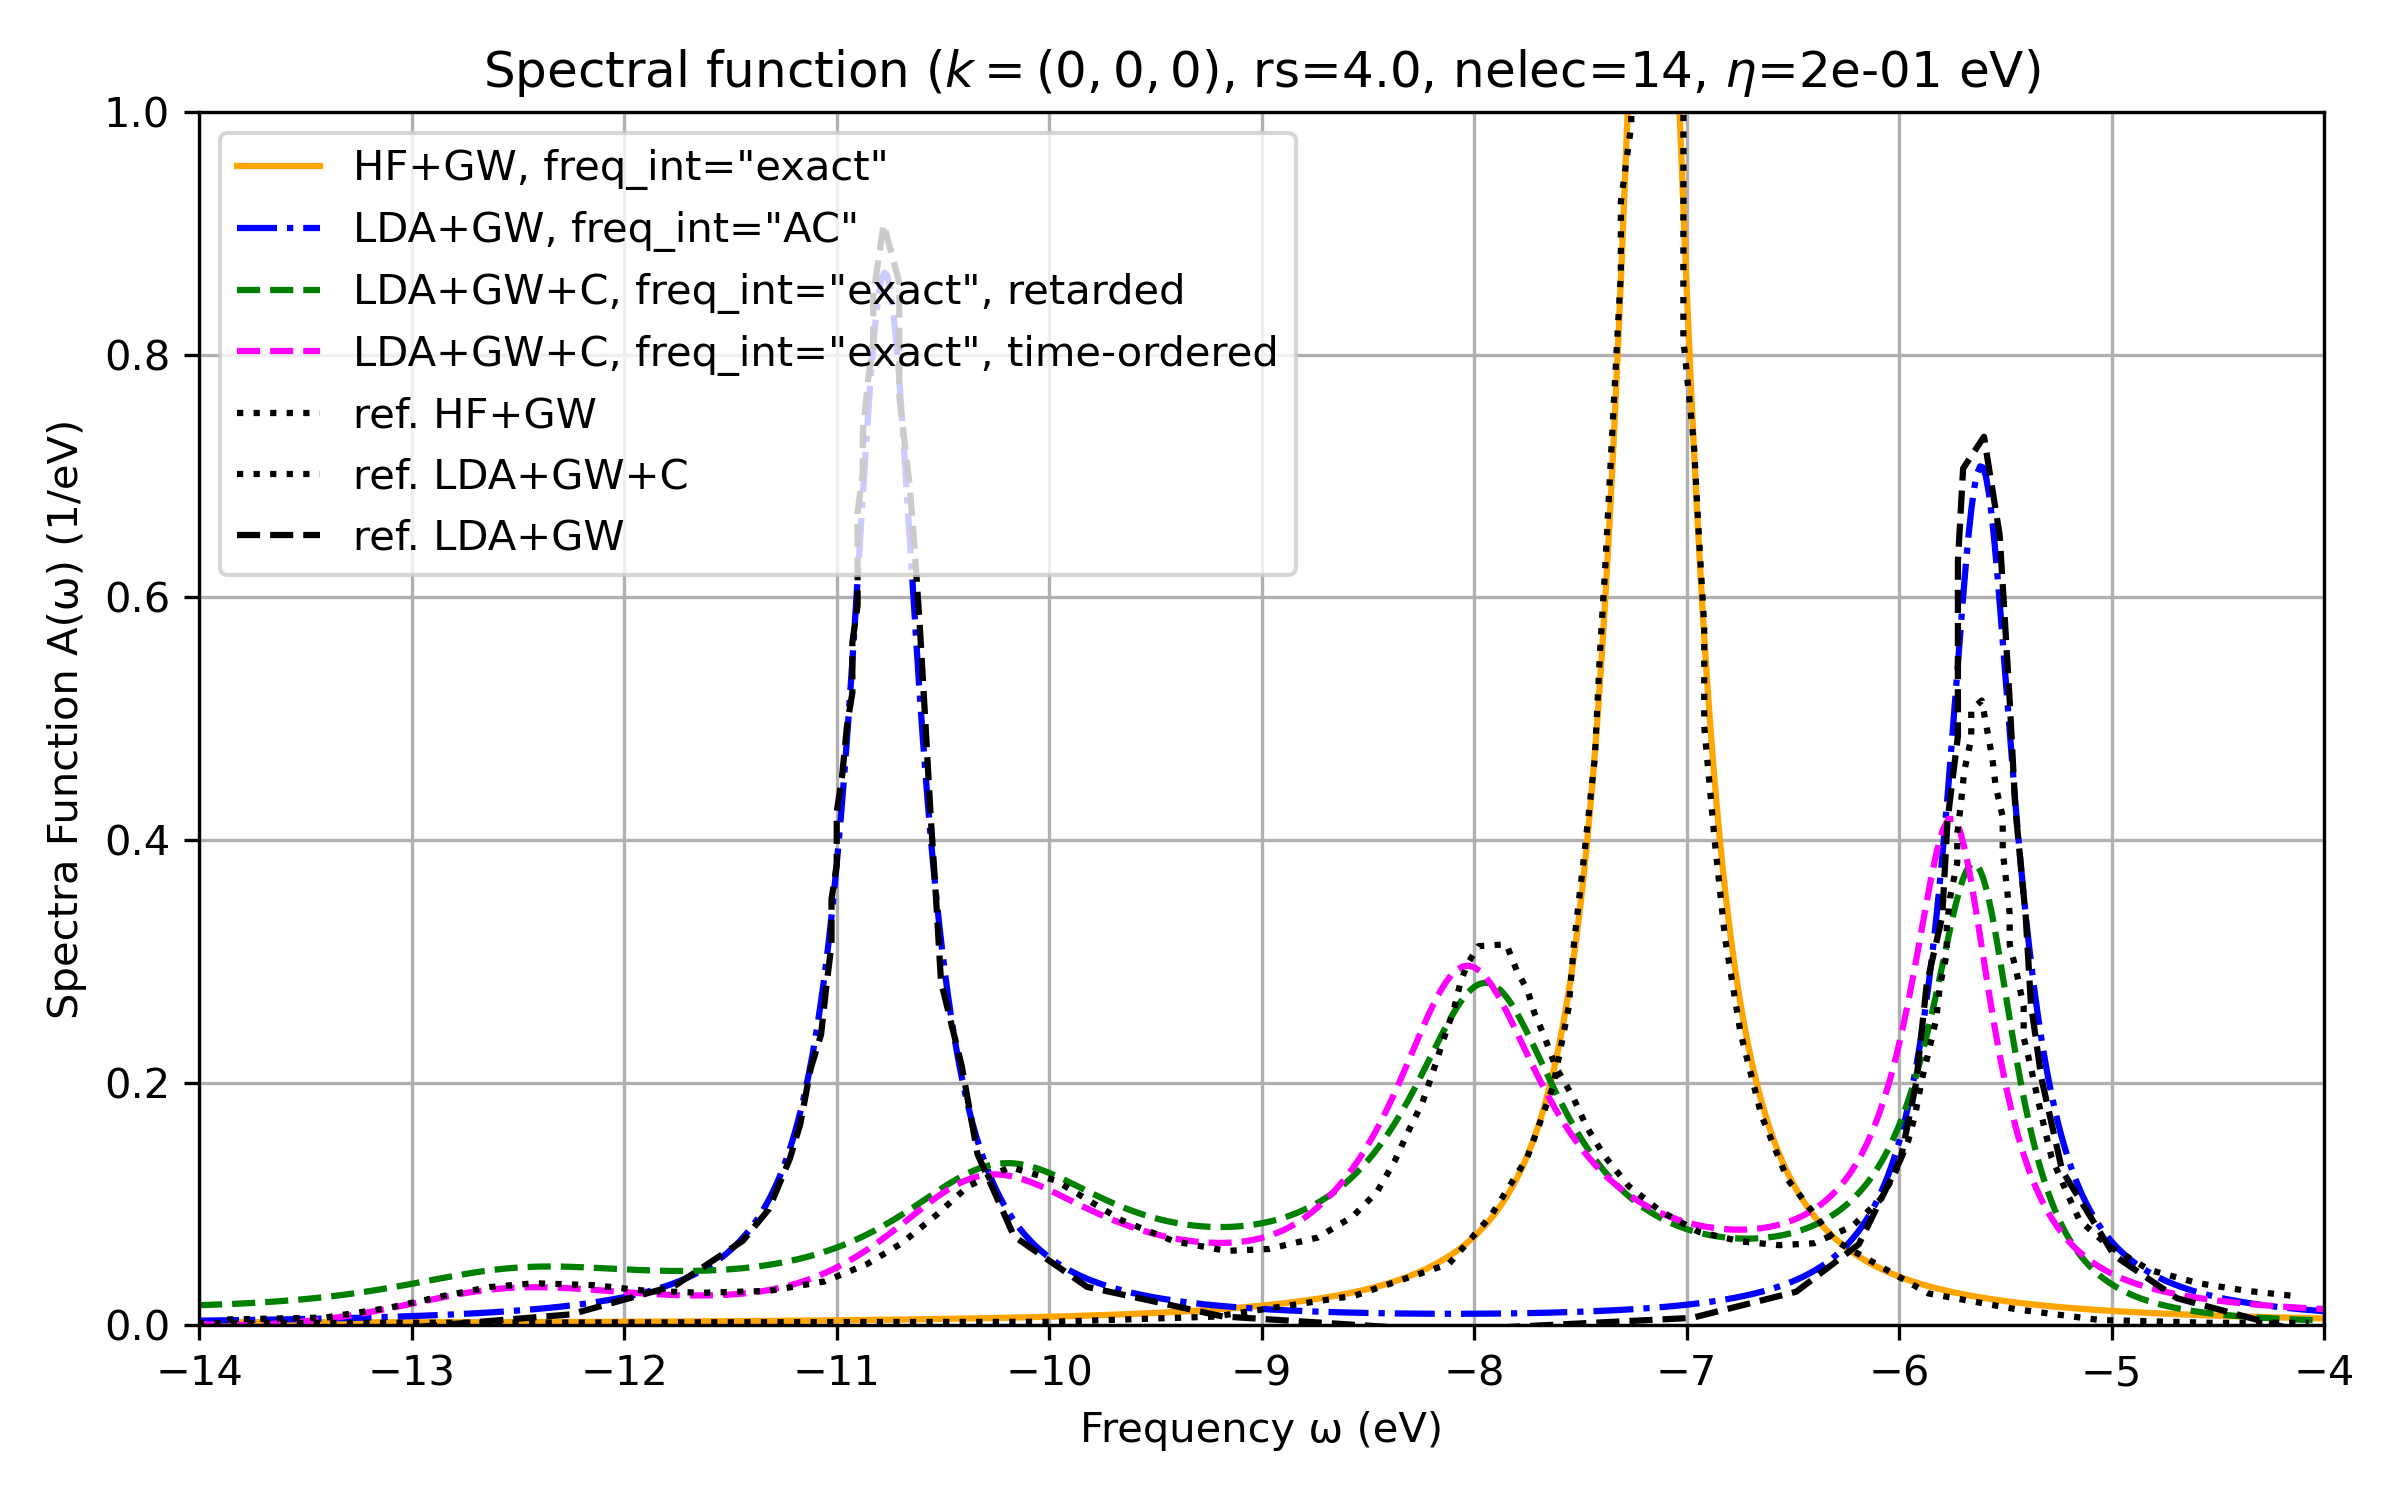
\includegraphics[width=\textwidth]{figs/image.png}
\end{figure}
\end{frame}
\begin{frame}
\frametitle{State of 14e/19o plots cont.}
\begin{figure}
    \centering
    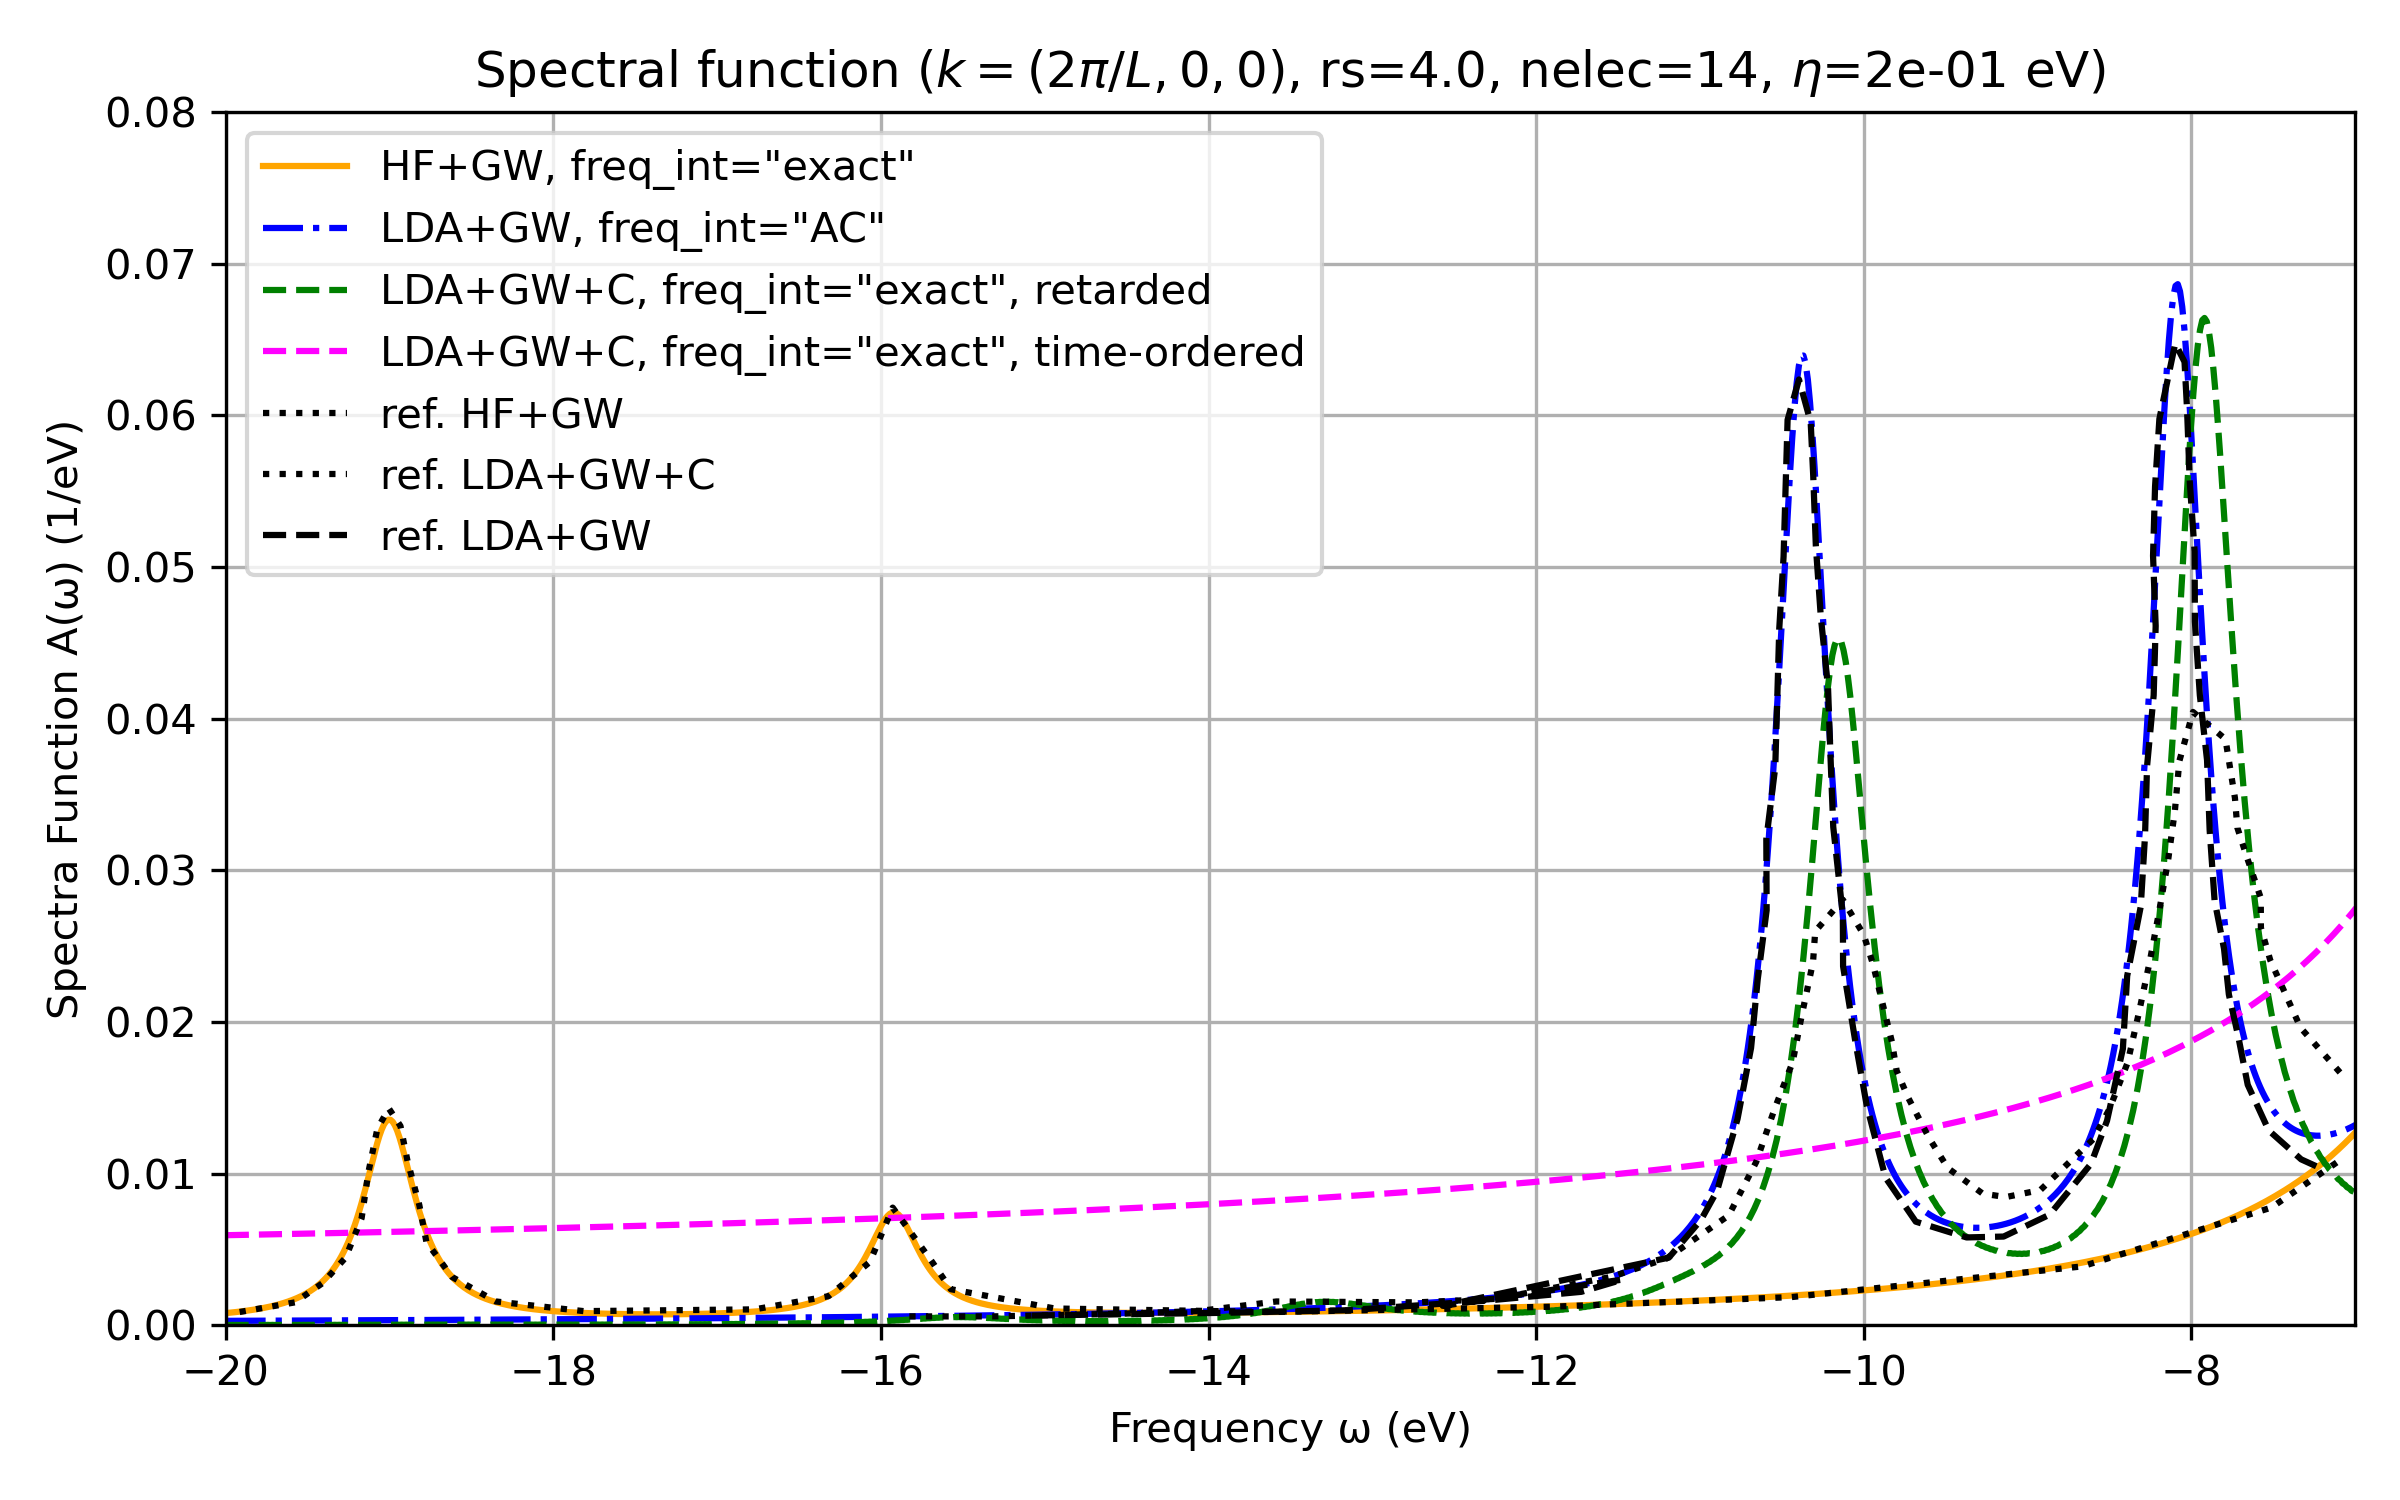
\includegraphics[width=\textwidth]{figs/v1_pidx6_rs4.0.png}
\end{figure}
\end{frame}
\begin{frame}
\frametitle{Time ordering}
\begin{align}
    A_{k}(\omega)
 & =\frac{1}{\pi}\left|\operatorname{Im} G_{k}^{\mathrm{T}}(\omega)\right|=-\frac{1}{\pi} \operatorname{Im} G_{k}^{\mathrm{R}}(\omega)
\end{align}
\pause
Retarded:
\begin{align}
    G^R_k(t)&= G^R_{0, k}(t) \exp \left[-i \Sigma_k^{\mathrm{x}} t+C^R_k(t)\right] \\
C^R_k(t) & =\pi^{-1} \int d \omega\left|\operatorname{Im} \Sigma^R_k\left(\omega+E_k^{G W}\right)\right|\left(e^{-i \omega t}+i \omega t-1\right) / \omega^2
\end{align}
\pause
vs. time ordered:
\begin{align}
    G_{k}^{\mathrm{T}}(t)&=\mathrm{i} \Theta(-t) e^{-\mathrm{i} \epsilon_k t} e^{C_{ k}^{\mathrm{T}}(t)} \\
C_{k}^{\mathrm{T}}(t) & =\int d \omega \frac{\beta_k^{ -}(\omega)}{\omega^2}\left(e^{-i \omega t}+i \omega t-1\right)\\
\beta_k^{ -}(\omega) & = \left|\operatorname{Im} \Sigma_k^R\left(\omega+\epsilon_k\right)\right| \theta\left[-\left(\epsilon_{k_F}-\epsilon_k-\omega\right)\right]
\end{align}
\end{frame}
\begin{frame}
\frametitle{Plasmon-pole model}
\begin{equation}
\Sigma^c(\mathbf{k}, \omega)=\sum_{\mathbf{q}} v(q) A(q)\left[\frac{1-f_{\mathbf{k}-\mathbf{q}}}{\omega-\varepsilon_{\mathbf{k}-\mathbf{q}}-\tilde{\omega}(q)+i \eta}+\frac{f_{\mathbf{k}-\mathbf{q}}}{\omega-\varepsilon_{\mathbf{k}-\mathbf{q}}+\tilde{\omega}(q)+i \eta}\right]
\end{equation}
\pause
with 
\begin{align}
A(q) &=-\frac{\pi}{2} \frac{\Omega(q)}{\tilde{\omega}(q)} \\
\Omega(q)^2
&= 4\pi n \\
\tilde{\omega}(q)^2 &= \frac{\Omega(q)^2}{1 - \epsilon^{-1}(q, \omega=0)} \\
\operatorname{Re} \epsilon^{-1}(q, \omega) &\approx 1+\frac{\Omega(q)^2}{\omega^2-\tilde{\omega}(q)^2}
\end{align}
\pause
Do we need finite-size corrections?
\end{frame}
\section{Future directions}
\begin{frame}
\frametitle{Future directions}
\begin{itemize}
    \item Verify that doing plasmon-pole model for the frequency integration reproduces the reference
    \pause
    \item Implement additional frequency integration schemes
\end{itemize}
\end{frame}
% \section{PPM deviates from AC}
\begin{frame}
    \frametitle{114e/485o}
    \begin{figure}
        \centering
        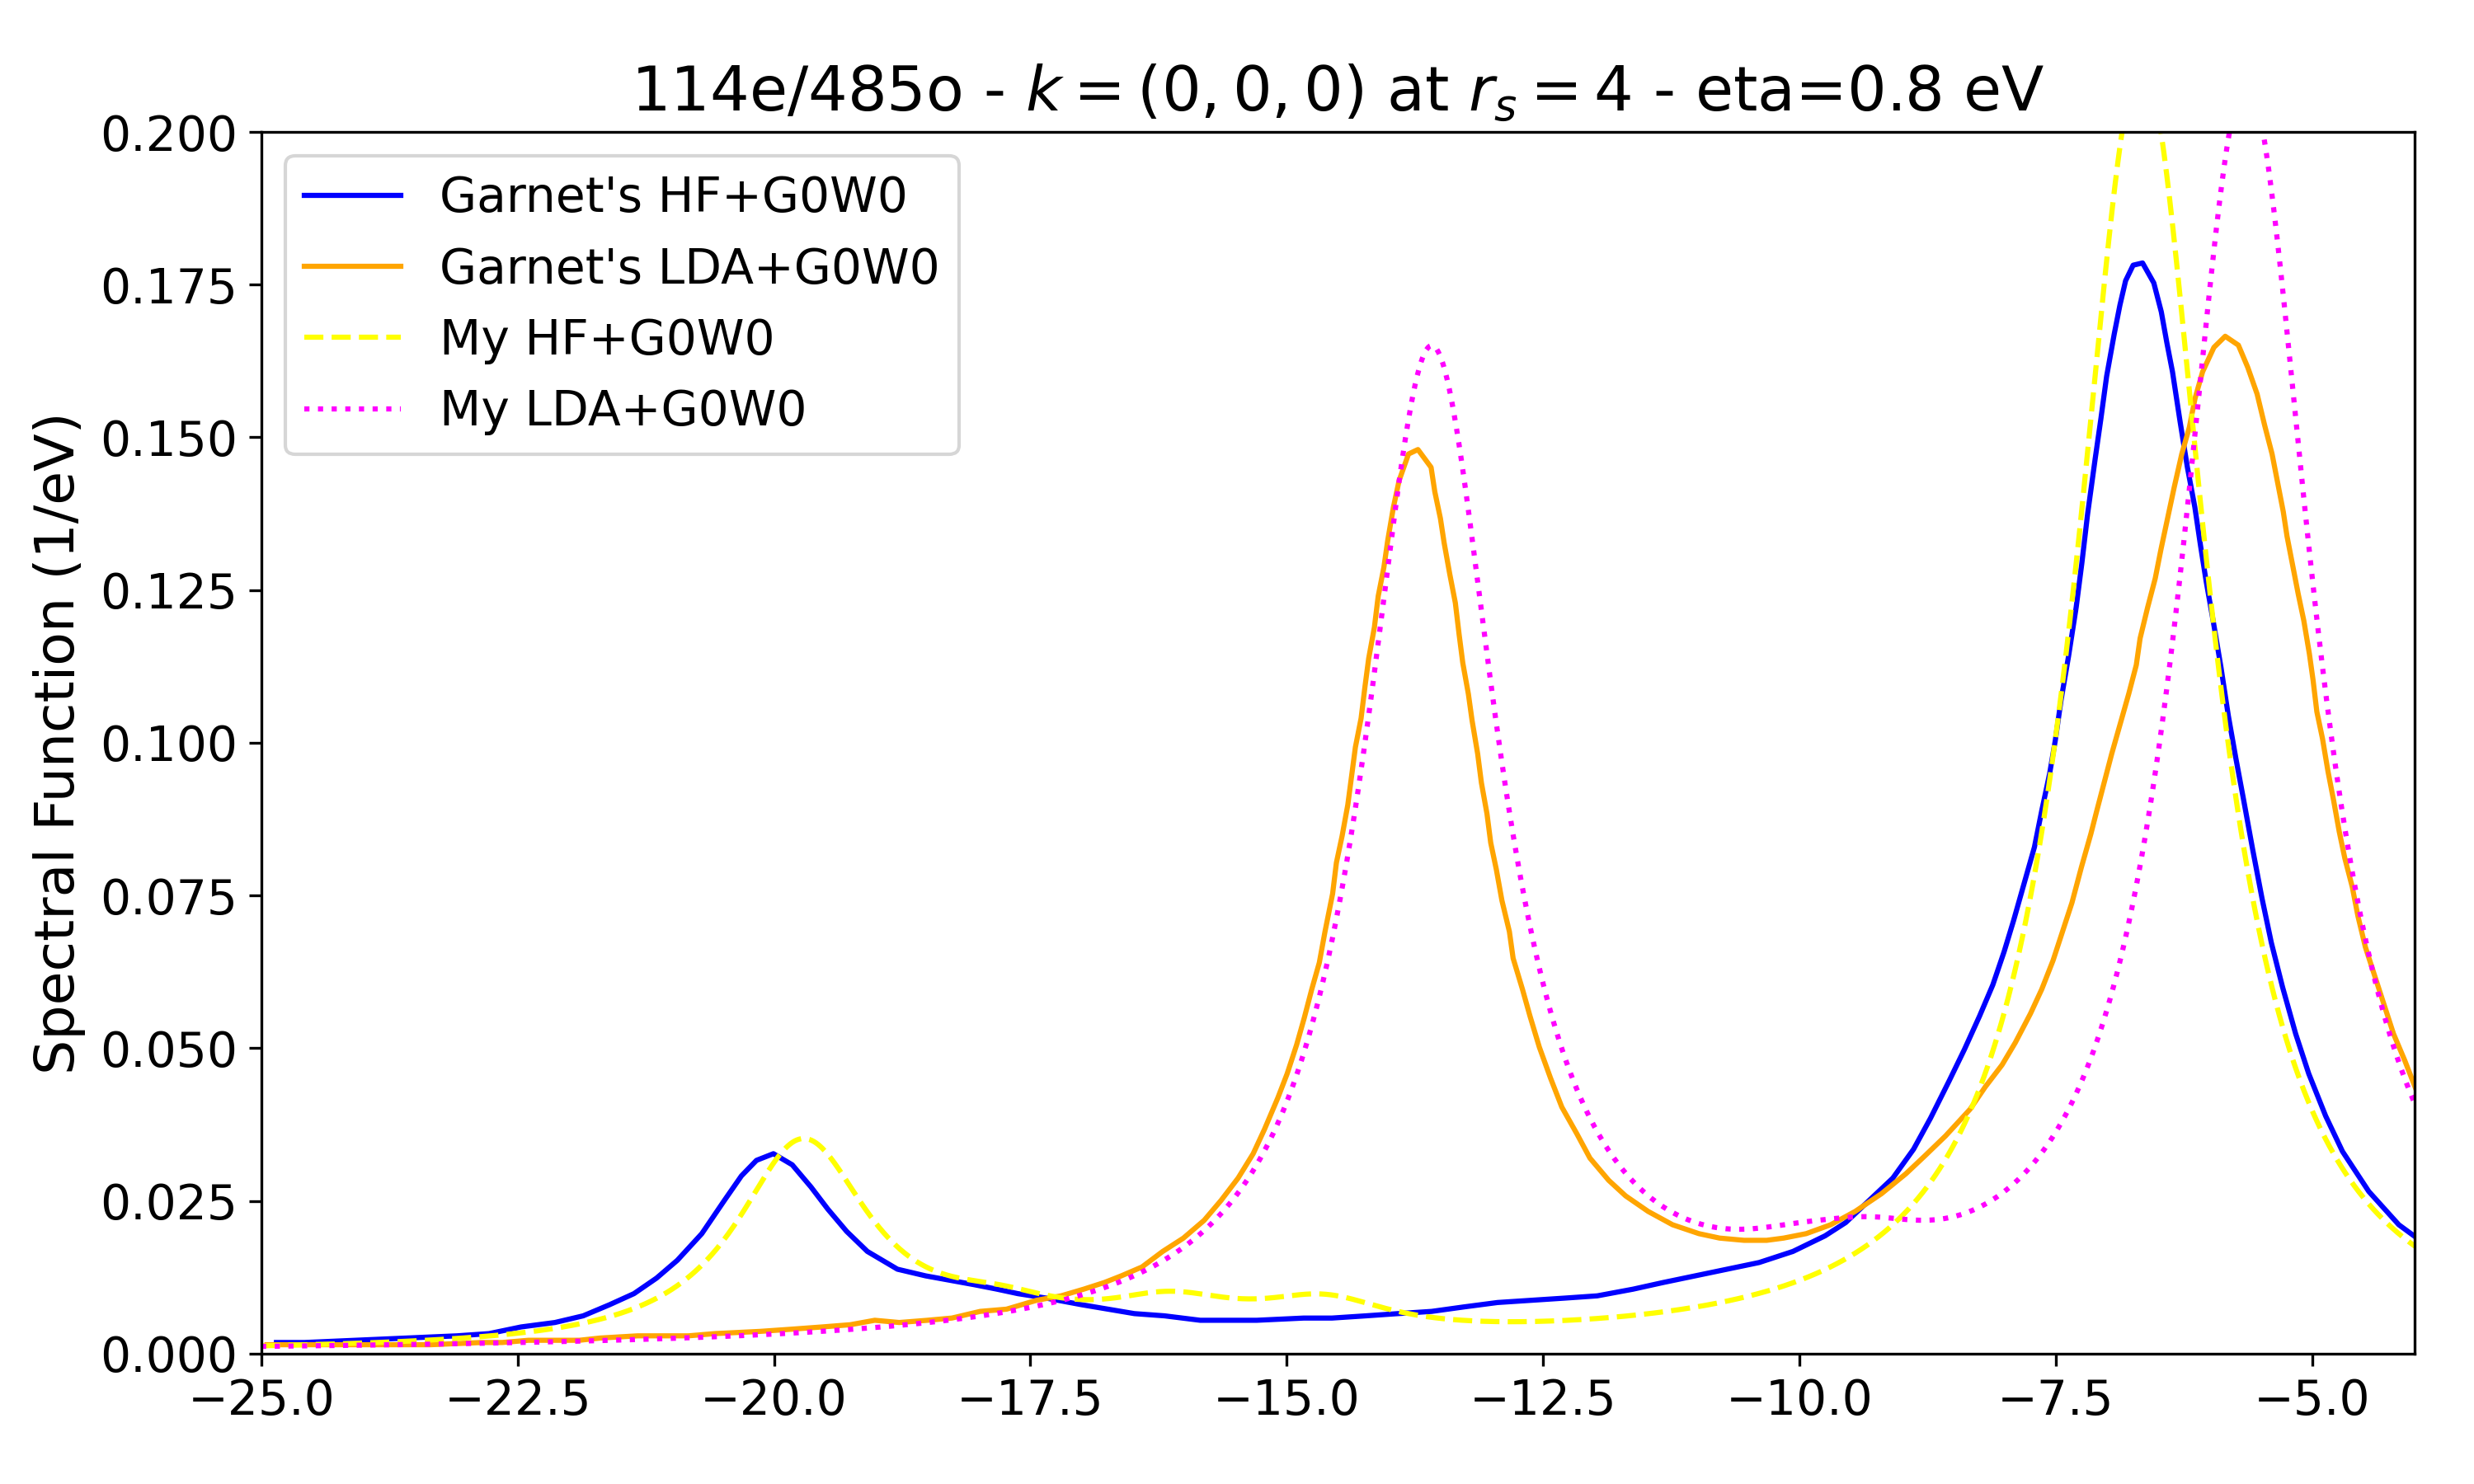
\includegraphics[width=\textwidth]{figs/6-12/refpgw.png}
    \end{figure}
\end{frame}
\begin{frame}
    \frametitle{14e/57o}
    \begin{figure}
        \centering
        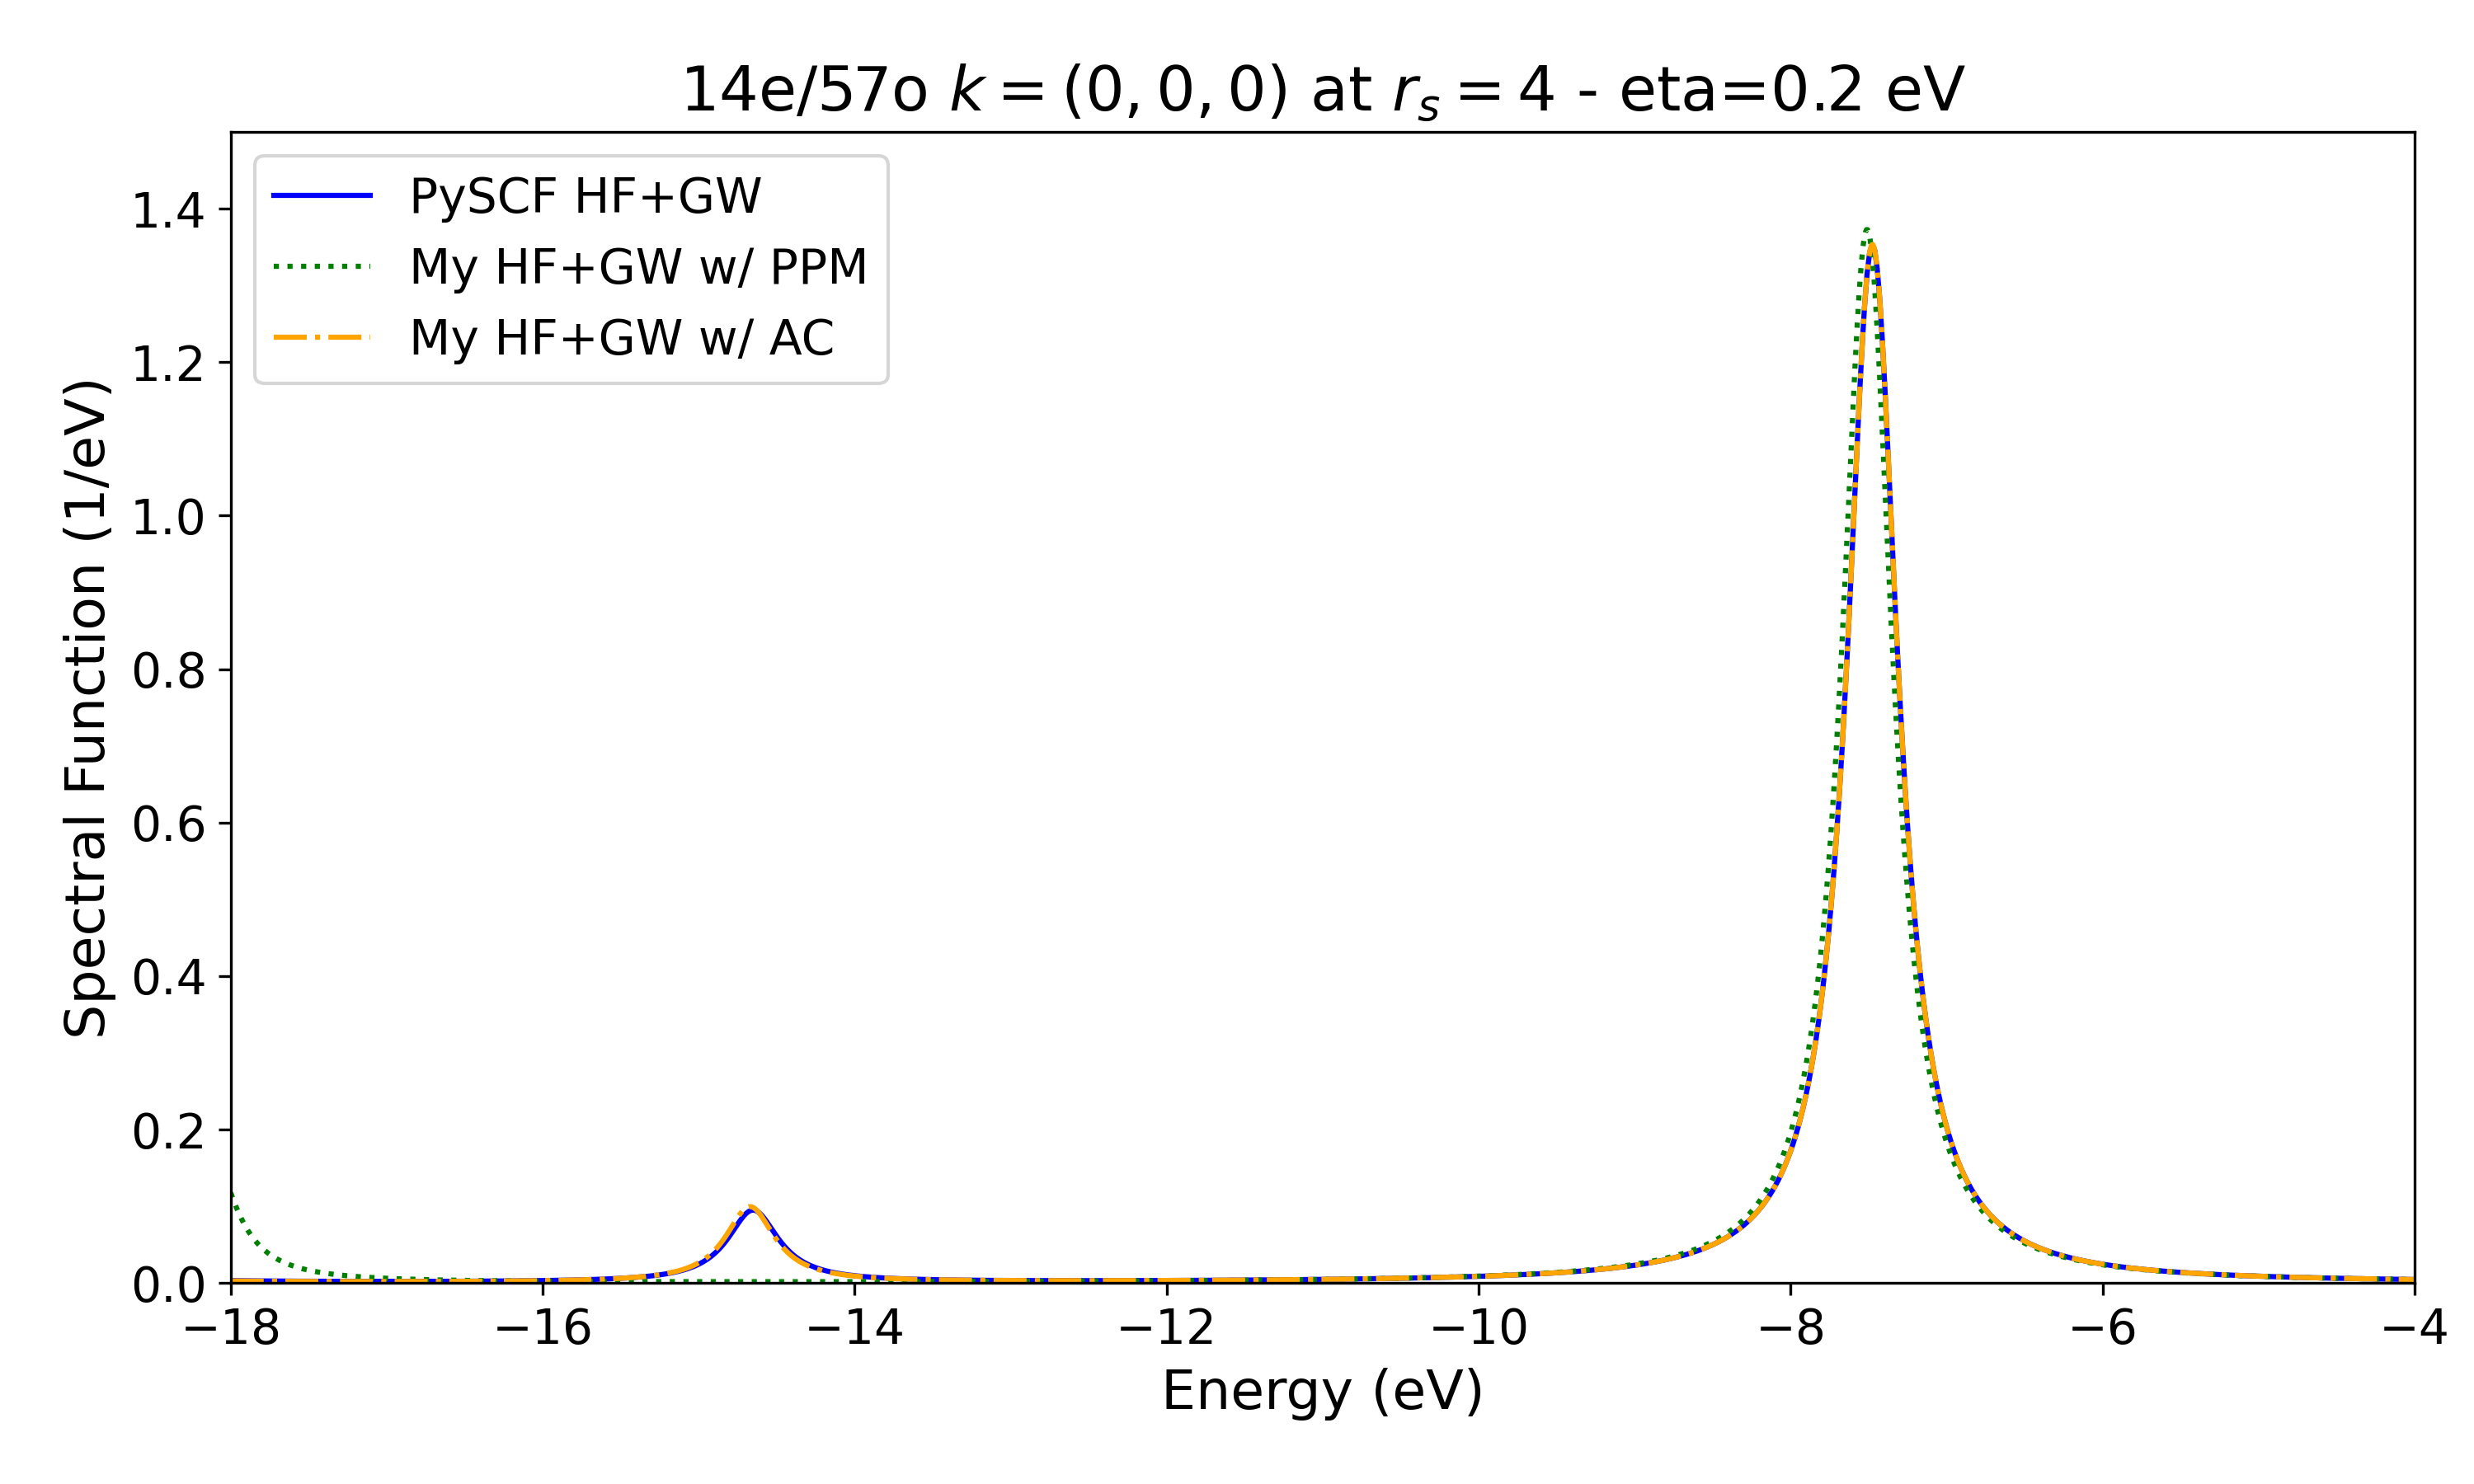
\includegraphics[width=\textwidth]{figs/6-12/gw_14e57o.png}
    \end{figure}
\end{frame}
\section{Why I don't think AC is the right answer}
\begin{frame}
    \frametitle{Theory}
\begin{align}
    \Sigma_{n n^{\prime}}^c(\mathbf{k}, i \omega)&= -\frac{1}{\pi N_{\mathbf{k}}} \sum_{m \mathbf{q}} \int_0^{\infty} d \omega^{\prime} \frac{i \omega+\epsilon_F-\epsilon_{m \mathbf{k}-\mathbf{q}}}{\left(i \omega+\epsilon_F-\epsilon_{m \mathbf{k}-\mathbf{q}}\right)^2+\omega^{\prime 2}}\\
&\times  \sum_{P Q} v_P^{n m}\left[\left[\mathbf{I}-\mathbf{\Pi}\left(\mathbf{q}, i \omega^{\prime}\right)\right]_{P Q}^{-1}-\delta_{P Q}\right] v_Q^{m n^{\prime}}
\end{align}\pause
with the polarizability given by
\begin{equation}
\boldsymbol{\Pi}_{P Q}\left(\mathbf{q}, i \omega^{\prime}\right)=\frac{2}{N_{\mathbf{k}}} \sum_{\mathbf{k}} \sum_i^{\text {occ }} \sum_a^{\text {vir }} v_P^{i a} \frac{\epsilon_{i \mathbf{k}}-\epsilon_{a \mathbf{k}-\mathbf{q}}}{\omega^{\prime 2}+\left(\epsilon_{i \mathbf{k}}-\epsilon_{a \mathbf{k}-\mathbf{q}}\right)^2} v_Q^{a i}.
\end{equation}\pause
Then form Pade approximants as
\begin{equation}
    \Sigma_{n n^{\prime}}(\mathbf{k}, \mathbf{z})=\frac{a_0+a_1 \cdot \mathbf{z}+\ldots+a_{(N-1) / 2} \cdot z^{(N-1) / 2}}{1+b_1 \cdot \mathbf{z}+\ldots+b_{N / 2} \cdot z^{N / 2}}
\end{equation}\pause
and then analytically continue to the real axis.
\end{frame}
\begin{frame}
    \frametitle{38e/123o example}
    \begin{figure}
        \centering
        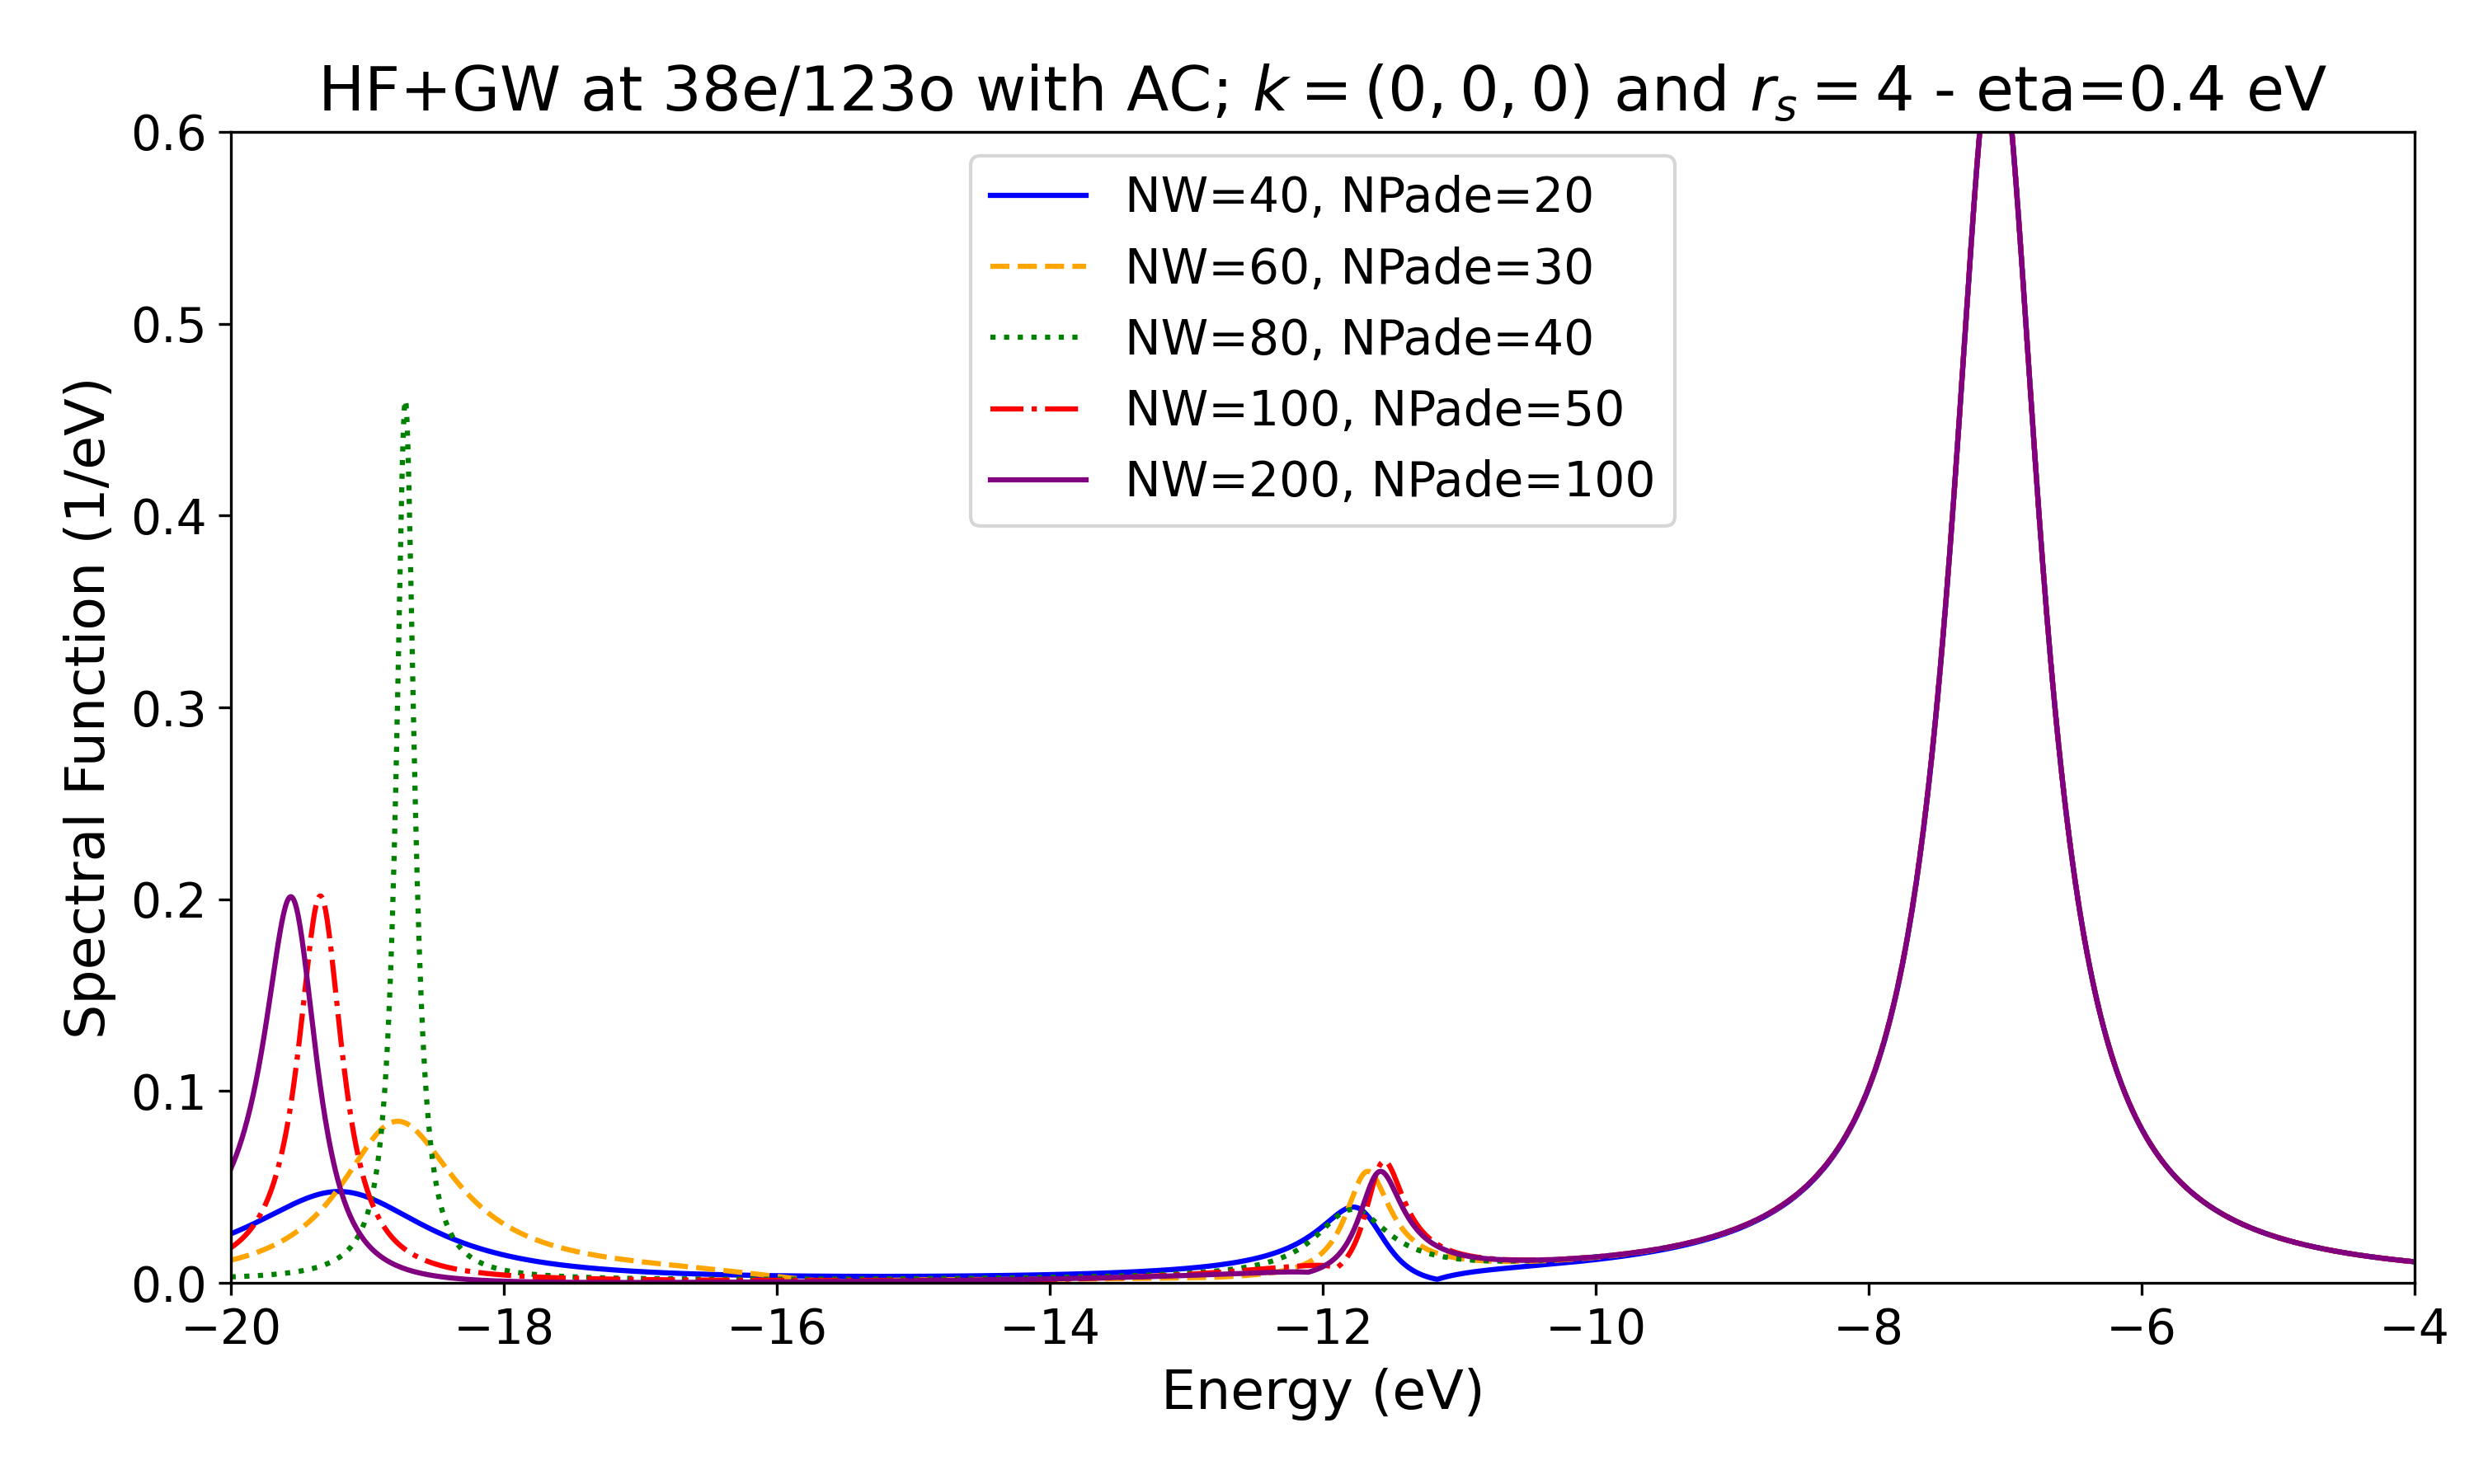
\includegraphics[width=\textwidth]{figs/6-12/gw_38e123o_ac.png}
    \end{figure}
\end{frame}
\begin{frame}
    \frametitle{Why using AC would be problematic for us}
\begin{itemize}
    \item Known to be numerically unstable for QP energies of deep core states. \pause
    \item Getting satellite features even more difficult. \pause
    \item Looked good for 14e/19o because this wasn't a true core state? \pause
    \item Need to run CD alongside AC and PPM for 114e/485o to verify this. 
\end{itemize}
\end{frame}
\begin{frame}
    \frametitle{Contour deformation for 14e/19o}
    \begin{figure}
        \centering
        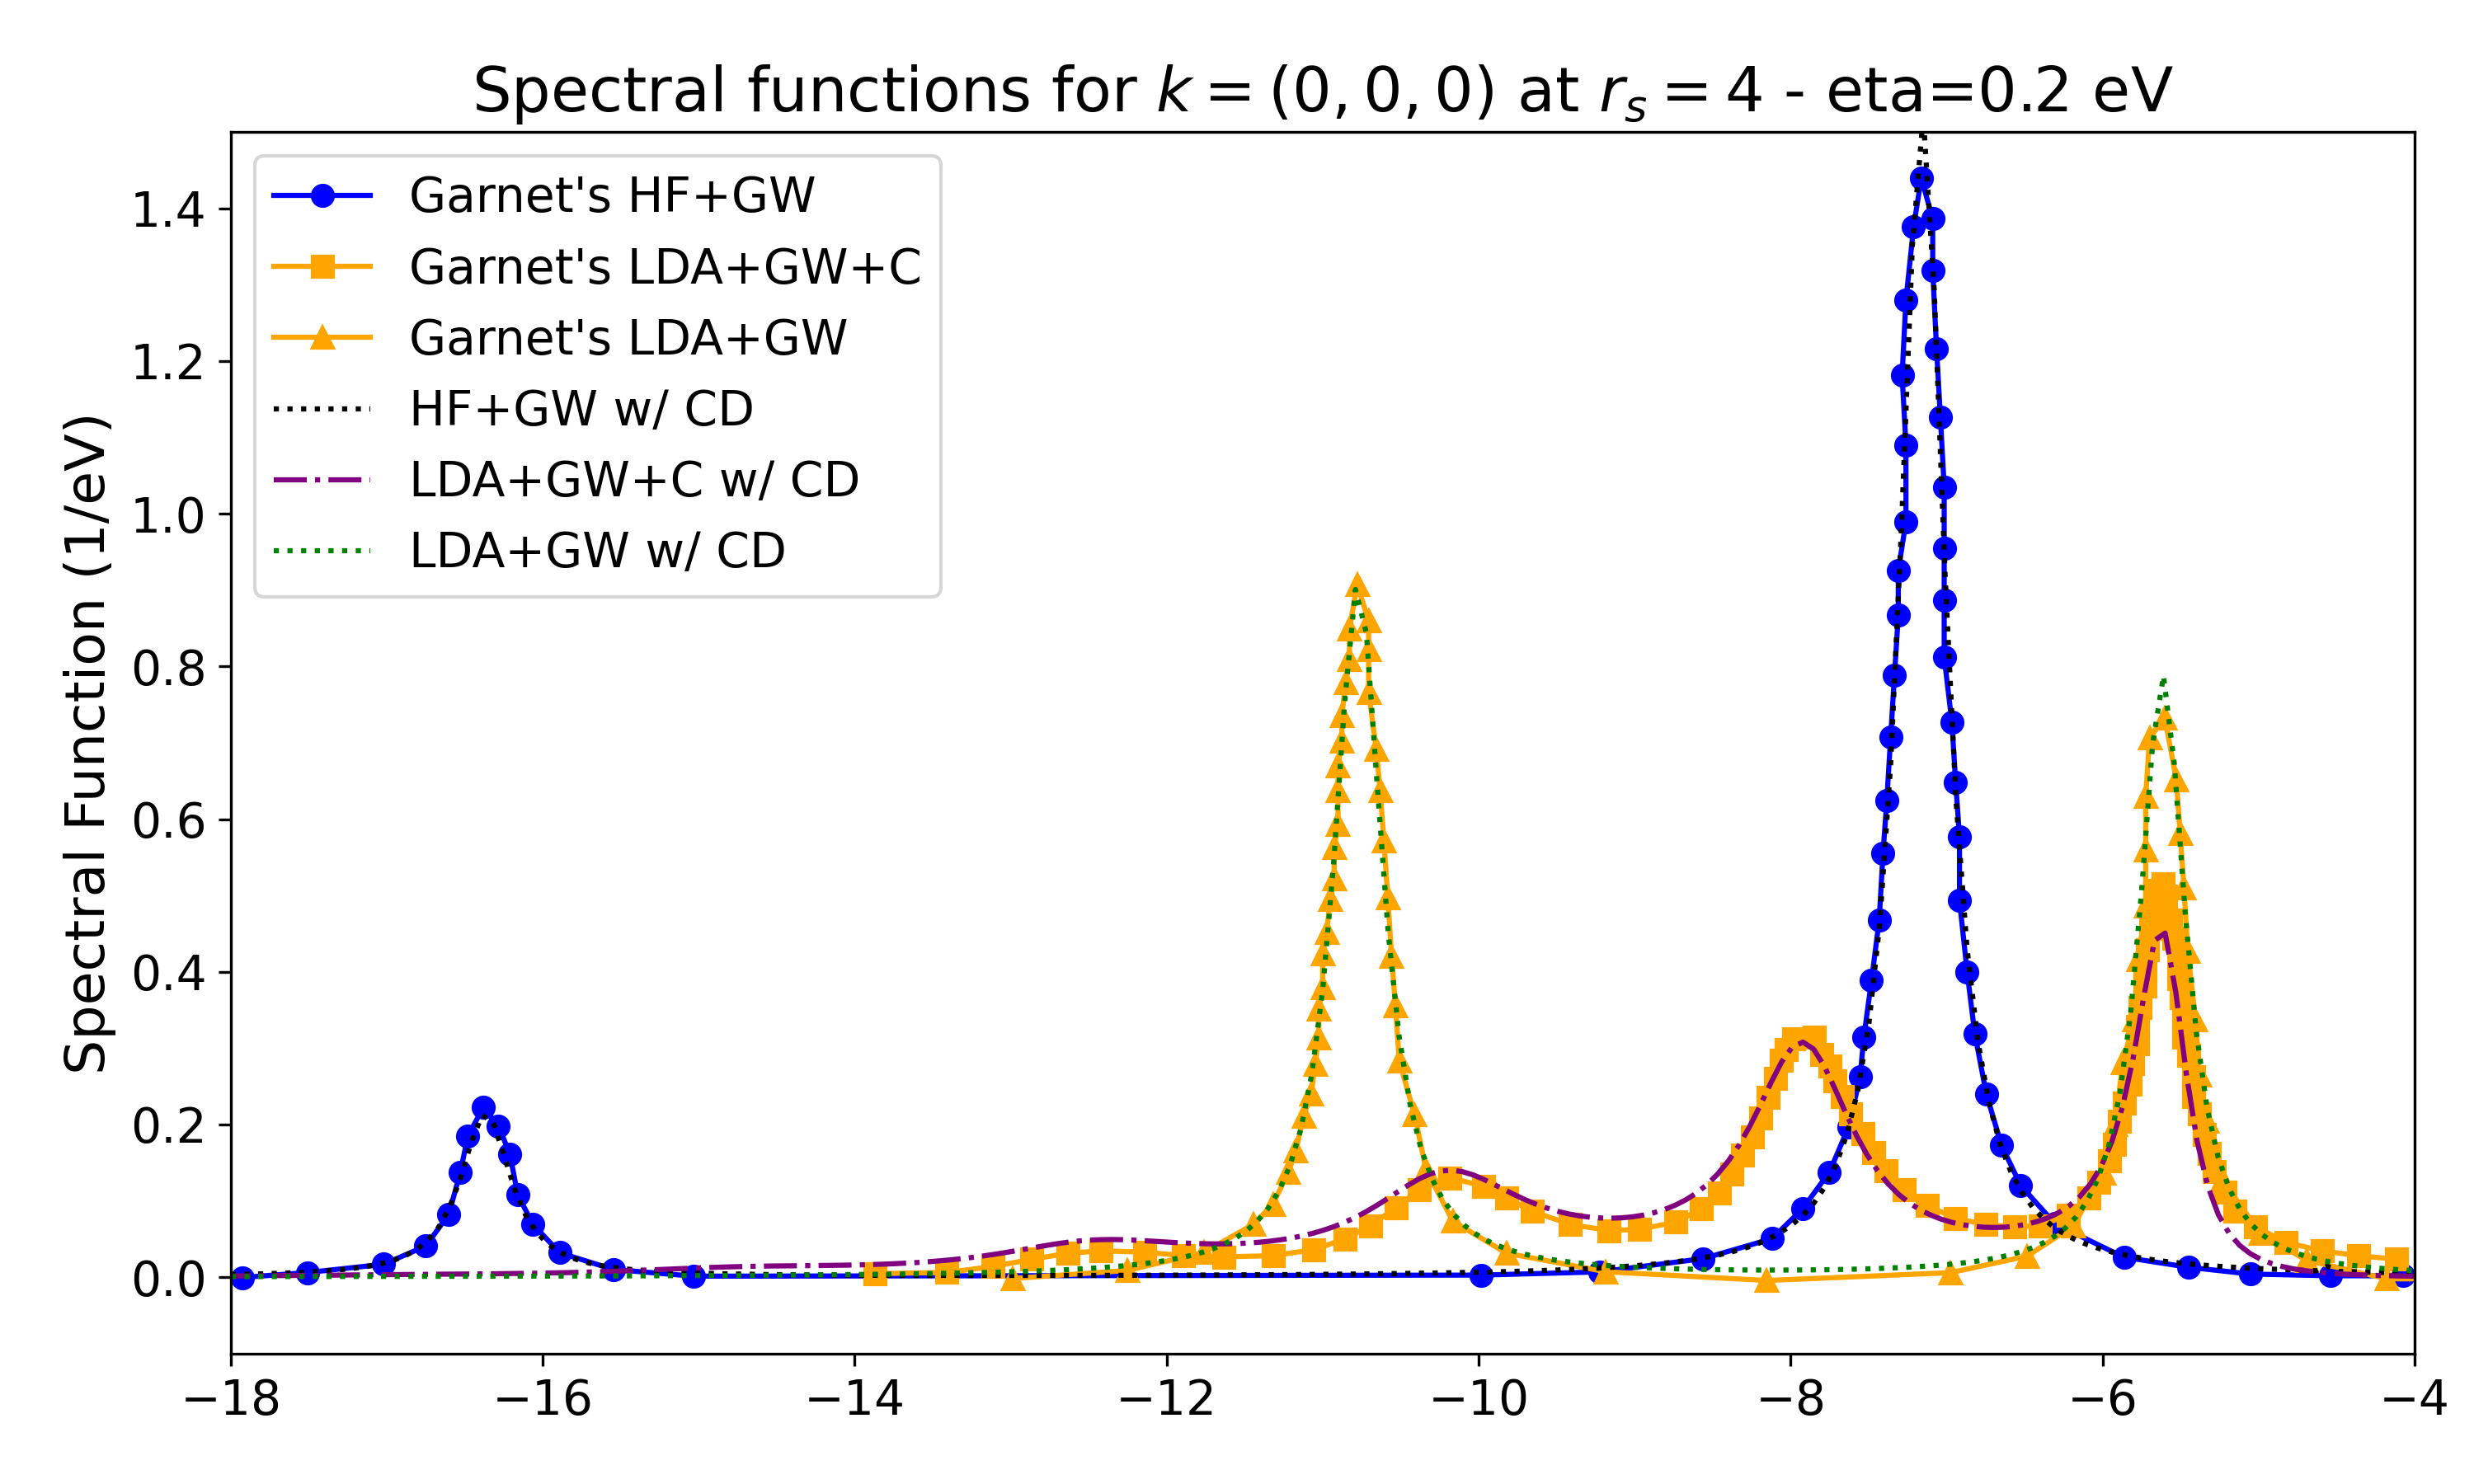
\includegraphics[width=\textwidth]{figs/6-12/gw_cd_verification.png}
    \end{figure}
\end{frame}
\section{Open questions}
\begin{frame}
    \frametitle{Open questions}
\begin{itemize}
    \item Should I spend time figuring out the bug in my PPM code? \pause
    \item Bad idea to run the $O(N^6)$ Casida diagonalization for 114e/485o?
\end{itemize}
\end{frame}

% \section{Updates}
\begin{frame}
    \frametitle{My previous plots overbroadened BWs2+C}
    \begin{figure}
        \centering
        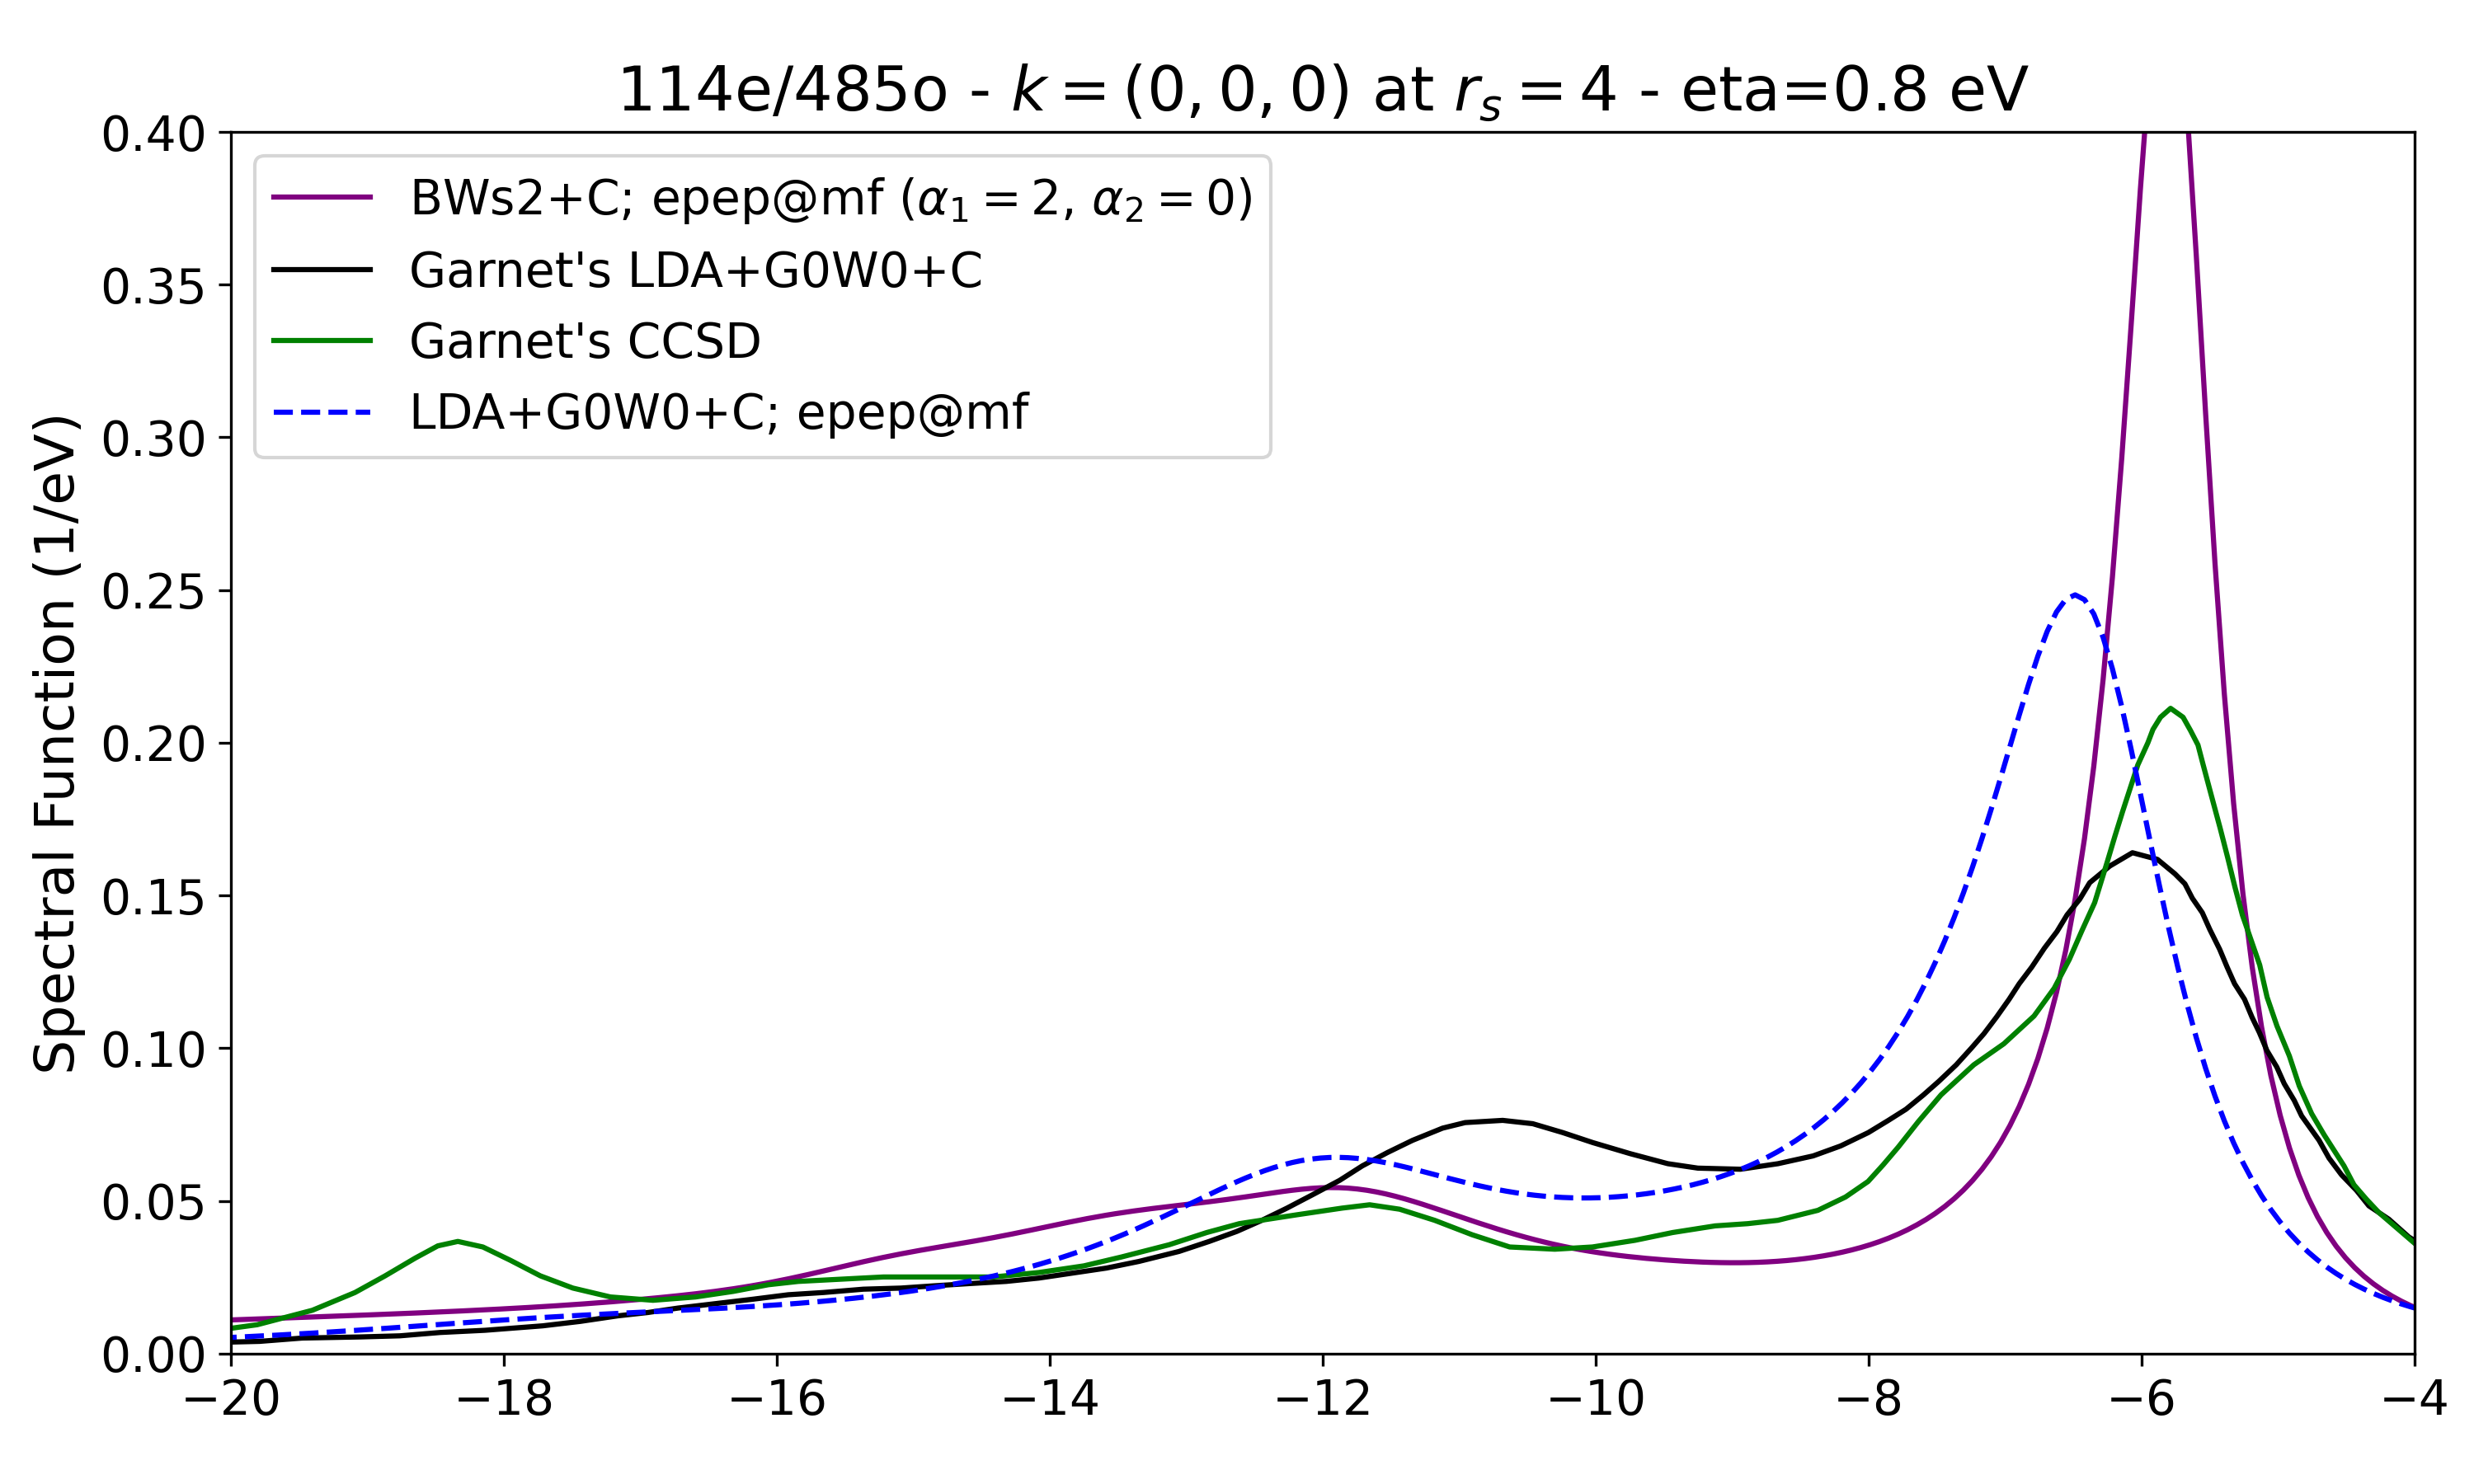
\includegraphics[width=\textwidth]{26/7/7-31/refpgw.png}
        % \caption{LDA+GW}
    \end{figure}
\end{frame}
\begin{frame}
    \frametitle{TDL comparison with references}
    \begin{figure}
        \centering
        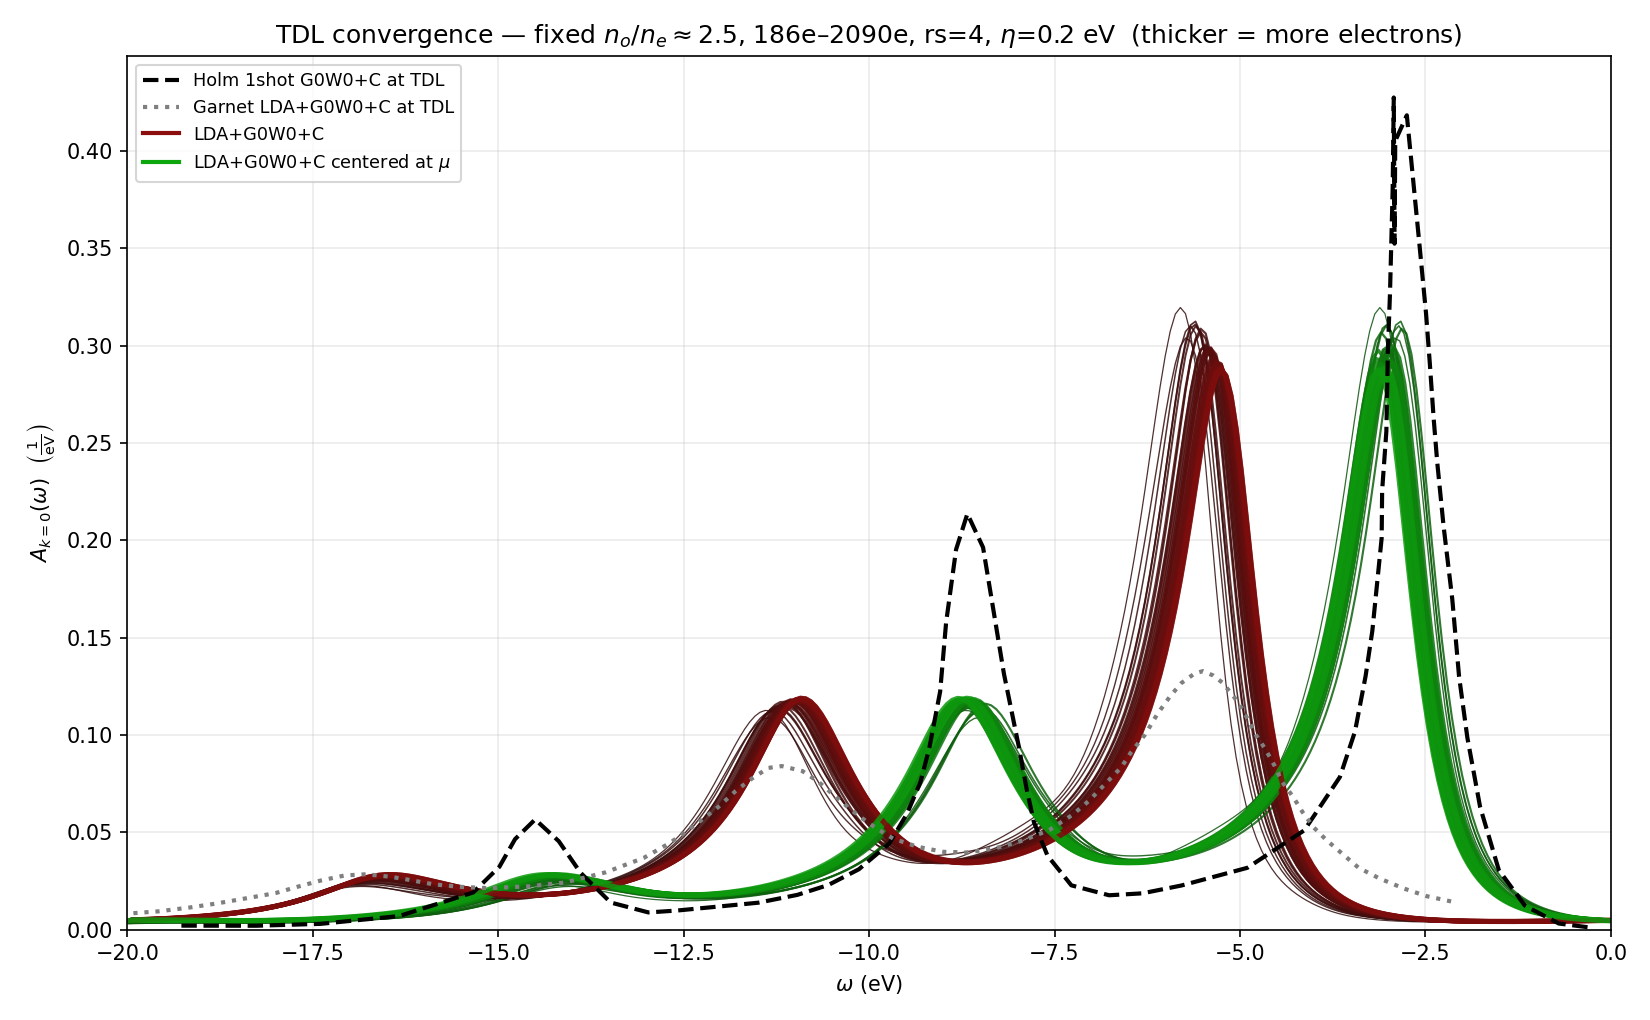
\includegraphics[width=\textwidth]{26/7/7-31/tdl_stream_overlay.png}
        % \caption{LDA+GW}
    \end{figure}
\end{frame}
\begin{frame}
    \frametitle{TDL convergence}
    \begin{figure}
        \centering
        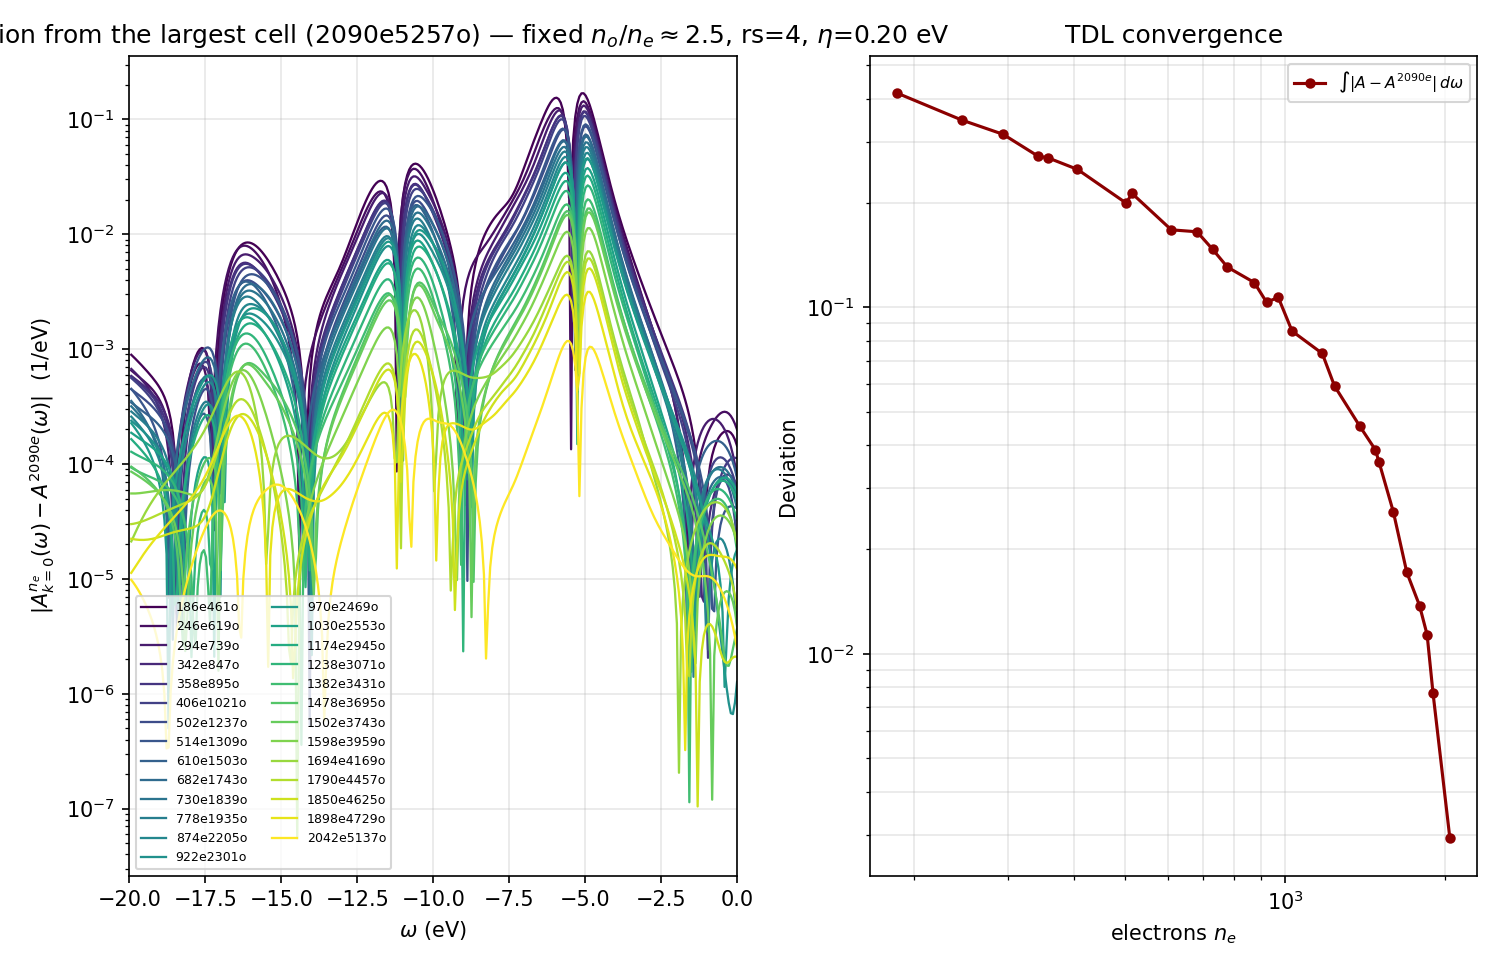
\includegraphics[width=\textwidth]{26/7/7-31/tdl_stream_diff.png}
        % \caption{LDA+GW}
    \end{figure}
\end{frame}

\section{SCCE(GW0) in a finite basis}
\begin{frame}
    \frametitle{Holms' paper}
    \begin{itemize}
        \item Fitting to Gaussians isn't practical for finite broadening \pause
        \item Landau form remains central
    \end{itemize}
\end{frame}
\begin{frame}
    \frametitle{Insights from reorganizing the Landau form}
\begin{align}
    C_{k}^R(t) &= \int d\omega \frac{\beta_{k}(\omega)}{\omega^2} \left( e^{-i\omega t} + i\omega t - 1 \right) \\
&= \underbrace{\int d\omega \frac{\beta_{k}(\omega)}{\omega^2} \left( e^{-i\omega t} - 1 \right)}_{C_k^{sat}(t)} + i t \underbrace{\int d\omega \frac{\beta_{k}(\omega)}{\omega}}_{\Delta_k} \\
&= C_k^{sat}(t) + i \Delta_k t
\end{align}
\pause
Since $\Delta_k=-\operatorname{Re}\Sigma^c_k(E_k^{GW})$, we can write
\begin{align}
    G^{R}_{k}(t)
    &= -i \Theta(t) e^{-i(\epsilon_k + \operatorname{Re} \Sigma_{c, k}^R(E)) t} e^{C_k^{sat}(t)} \\
    &= -i \Theta(t) e^{-i(E_k^{QP}) t} e^{C_k^{sat}(t)}.
\end{align}

\end{frame}
\begin{frame}
    \frametitle{Self-consistent scheme}
After the initial iteration, self-energy updates become 
\begin{equation}
    \Sigma_{k, c}^R(t)=\theta(t)\left[-\sum_{m<k_F, I}\left|M_{ k, m}^I\right|^2 G_{m,CE}^{<}(t) e^{+i \Omega_I t} + \sum_{m>k_F, I}\left|M_{ k, m}^I\right|^2 G_{m,CE}^{>}(t) e^{-i \Omega_I t}\right]
\end{equation}
and then DFT to get $\Sigma_{k, c}^R(\omega)$. \pause We can try three schemes
\begin{enumerate}
    \item update $E_k^{QP} = \epsilon_k + \operatorname{Re} \Sigma_{c, k}^R(E_k^{QP})$, but keep $C_k^{sat}(t)$ fixed \pause
    \item update $\beta_k^{\text{sat}}(\omega)$ and thus also $C_k^{sat}(t)$, but keep $E_k^{QP}$ fixed \pause
    \item update both $E_k^{QP}$ and $C_k^{sat}(t)$ 
\end{enumerate}
\end{frame}
\section{Connection to CCGF}
\begin{frame}
    \frametitle{Ground State of the Electronic Polaron in the IBM}
Hamiltonian is 
\begin{equation}
H_{\rm ch}
=
E_{\rm ch}
+
\sum_\nu
\Omega_\nu Q_\nu^\dagger Q_\nu
+
\sum_\nu
\left(
M_\nu Q_\nu^\dagger
+
M_\nu^* Q_\nu
\right).
\end{equation}
\pause
The ground state of the electronic Poluron is a coherent state of QB operators $Q_\nu$ as
\begin{equation}
    |\Theta_{ch}\rangle = D(\beta)\left|0_{\mathrm{RPA}}\right\rangle.
\end{equation} 
\pause
The displacement operator is defined as
\begin{equation}
    D(\beta)=\exp \left[\sum_\mu\left(\beta_\mu Q_\mu^{\dagger}-\beta_\mu^* Q_\mu\right)\right] .
\end{equation}
where $\beta_\mu = -M_\mu / \Omega_\mu$.
\end{frame}
\begin{frame}
    \frametitle{Green's function of the electronic polaron}
Using the shifted QB operators
\begin{equation}
\widetilde Q_\nu
=
Q_\nu
- \beta_\nu
\qquad
\widetilde Q_\nu^\dagger
=
Q_\nu^\dagger
+
\beta_\nu^*,
\end{equation}
of which $\left|0_{\mathrm{RPA}}\right\rangle$ is a coherent state,
\pause we can rewrite the Hamiltonian as
\begin{equation}
H_{\rm ch}
=
E_{\rm pol}
+
\sum_\nu
\Omega_\nu
\widetilde Q_\nu^\dagger \widetilde Q_\nu ,
\end{equation}
where $E_{\rm pol}=E_{\rm ch}-\sum_\nu \Omega_\nu |\beta_\nu|^2$. \pause Then
\begin{align}
G^{QB,R}_{\rm ch}(t)
&=
-i \theta(t)
\left\langle 0_{\rm RPA} \right|
e^{-i H_{\rm ch} t}
\left|0_{\rm RPA}\right\rangle
\\
% &=-i \theta(t) e^{-i E_{\mathrm{pol}} t}\left\langle 0_{\mathrm{RPA}}\right| e^{-i \sum_\nu \Omega_\nu \tilde{Q}_\nu \tilde{Q}_\nu t}\left|0_{\mathrm{RPA}}\right\rangle \label{eq:G_ch_t} \\
% &=
% -i \theta(t)
% e^{-i E_{\rm pol} t}
% \exp
% \left[
% \sum_{\nu}
% |\beta_{\nu}|^2
% \left(
% e^{-i \Omega_{\nu} t}
% -
% 1
% \right)
% \right]
% \\
&=
-i \theta(t)
e^{-i E_{\rm pol} t}
\underbrace{
\exp
\left[
-\sum_{\nu} |\beta_{\nu}|^2
\right]
}_{Z_{\rm pol}}
\prod_{\nu}
\exp
\left[
|\beta_{\nu}|^2 e^{-i\Omega_{\nu} t}
\right]
\\
% &=
% -i \theta(t)
% Z_{\rm pol}
% e^{-i E_{\rm pol} t}
% \prod_{\nu}
% \sum_{n_{\nu}=0}^{\infty}
% \frac{
% |\beta_{\nu}|^{2n_{\nu}}
% }{
% n_{\nu}!
% }
% e^{-i n_{\nu} \Omega_{\nu} t}
% \\
&=
-i \theta(t)
Z_{\rm pol}
\sum_{\mathbf n}
\left[
\prod_{\nu}
\frac{
|\beta_{\nu}|^{2n_{\nu}}
}{
n_{\nu}!
}
\right]
\exp
\left[
-i
\left(
E_{\rm pol}
+
\sum_{\nu} n_{\nu}\Omega_{\nu}
\right)t
\right].
\end{align}
\end{frame}
\begin{frame}
    \frametitle{Connection between the cumulant and the CCGF in this formalism}
If instead of the IBM, we consider
\begin{equation}
H_p^{\rm eff}
=
\epsilon_p^{\rm HF}
+
\sum_{m\nu}
\Delta_{pm\nu}
B_{pm\nu}^{\dagger}
B_{pm\nu}
+
\sum_{m\nu}
\left(
\mathcal{M}_{pm\nu}
B_{pm\nu}^{\dagger}
+
\mathcal{M}_{pm\nu}^{*}
B_{pm\nu}
\right),
\end{equation}

then we recover the G0W0+C Green's function. \pause We can make contact with the CCGF, by instead considering the Hamiltonian
\begin{equation}
H_{\mathrm{ch}}=E_{\mathrm{ref}}^{\mathrm{ch}}+\sum_{p q} f_{p q}^{\mathrm{ch}}\left\{a_p^{\dagger} a_q\right\}+\frac{1}{4} \sum_{p q r s} v_{p q r s}^{\mathrm{ch}}\left\{a_p^{\dagger} a_q^{\dagger} a_s a_r\right\},
\end{equation}
which leads to the CCGF.
\end{frame}

% \section{Review of TDL extrapolations}
\begin{frame}
    \frametitle{LDA+GW}
    \begin{figure}
        \centering
        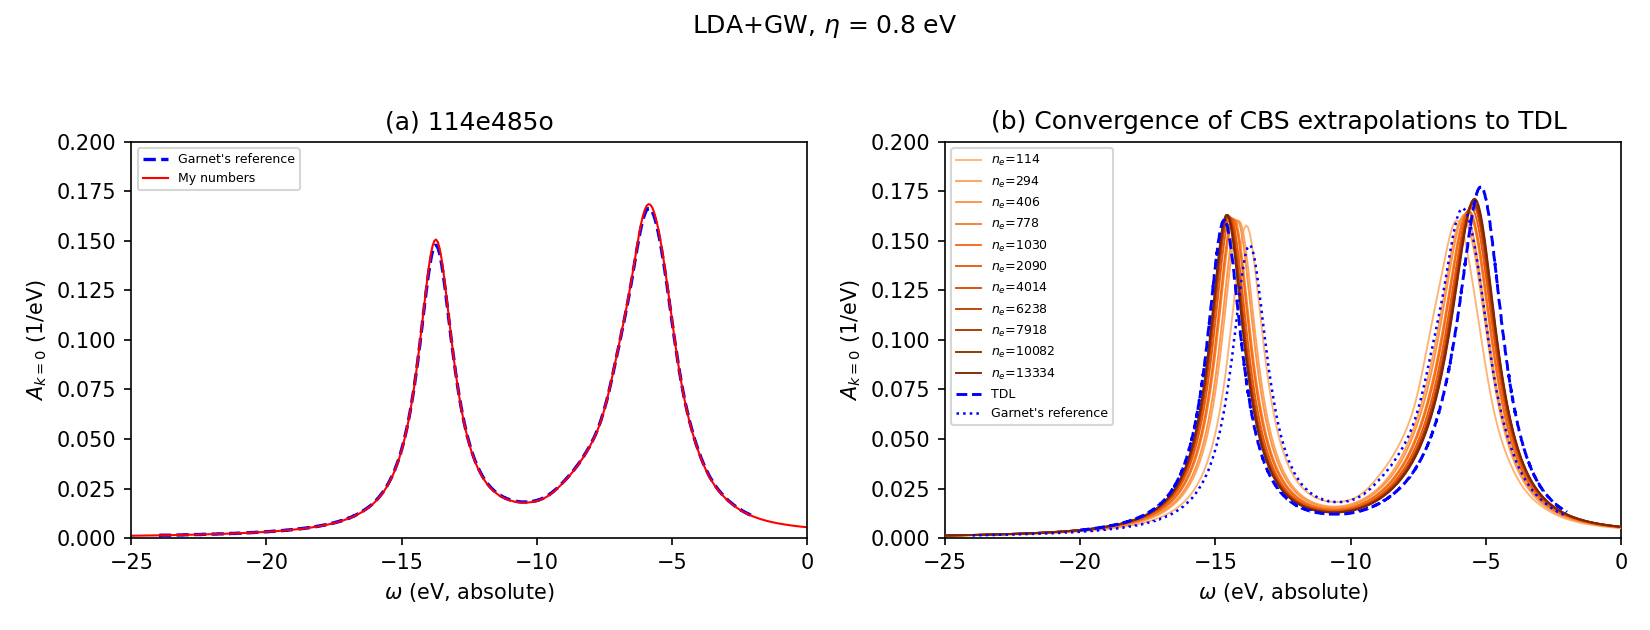
\includegraphics[width=\textwidth]{26/8/8-07/mcclain_compare.png}
        % \caption{LDA+GW}
    \end{figure}
\end{frame}
\begin{frame}
    \frametitle{LDA+GW+C Garnet's convention}
We are using 
\begin{equation}
    C_k^R(t) = \frac{1}{\pi}\int d\omega \frac{|\operatorname{Im} \Sigma^R_k(\omega+{E^{GW}_k})|}{\omega^2} \left( e^{-i\omega t} + i\omega t - 1 \right).
\end{equation}
\pause
    \begin{figure}
        \centering
        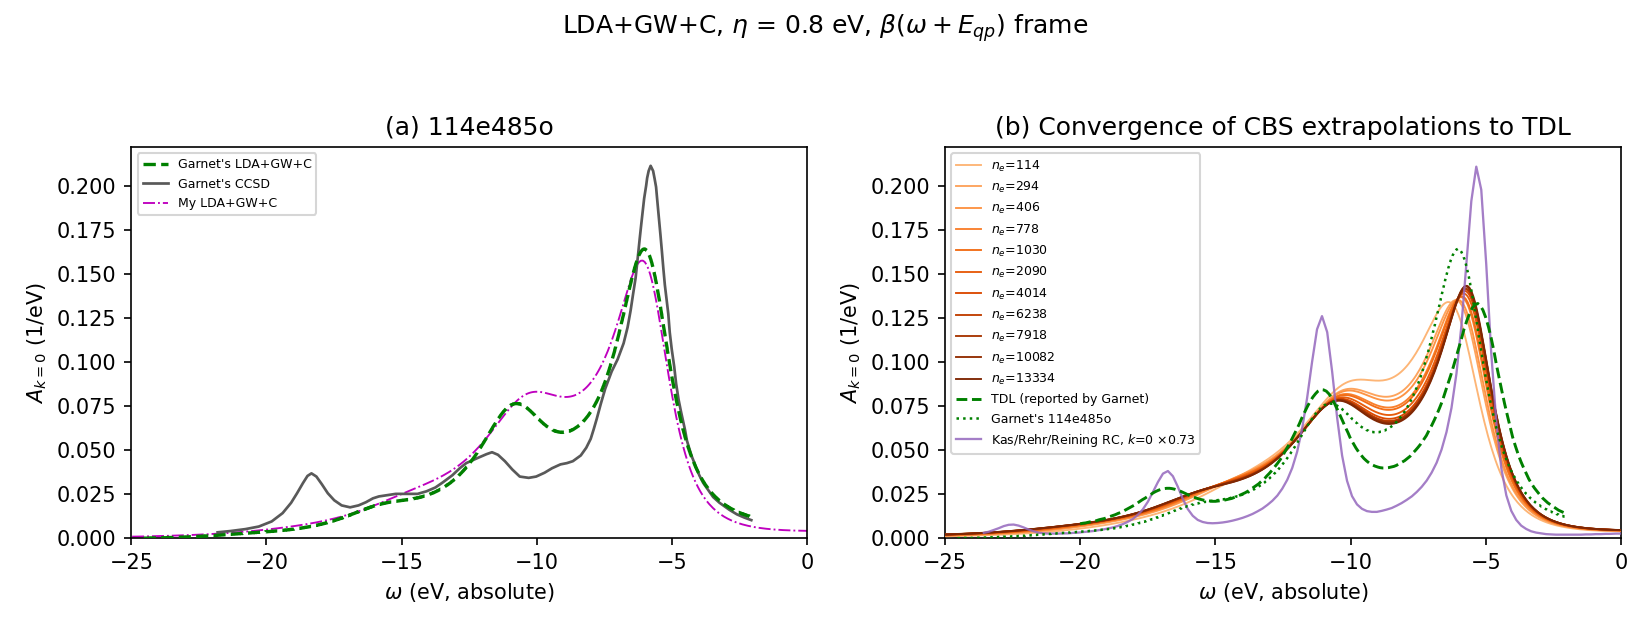
\includegraphics[width=\textwidth]{26/8/8-07/mcclain_gwc_compare_eqp.png}
        % \caption{LDA+GW}
    \end{figure}
% In the $\beta(\omega+E_{QP})$ and $\beta(\omega+\epsilon_{\mathrm{LDA}})$ frames, we are using $\epsilon_k \equiv E_k^{GW} $ and $\epsilon_k \equiv \epsilon_k^{\mathrm{LDA}}$, respectively.

\end{frame}
\begin{frame}
    \frametitle{LDA+GW+C Garnet's convention continued}
    \begin{figure}
        \centering
        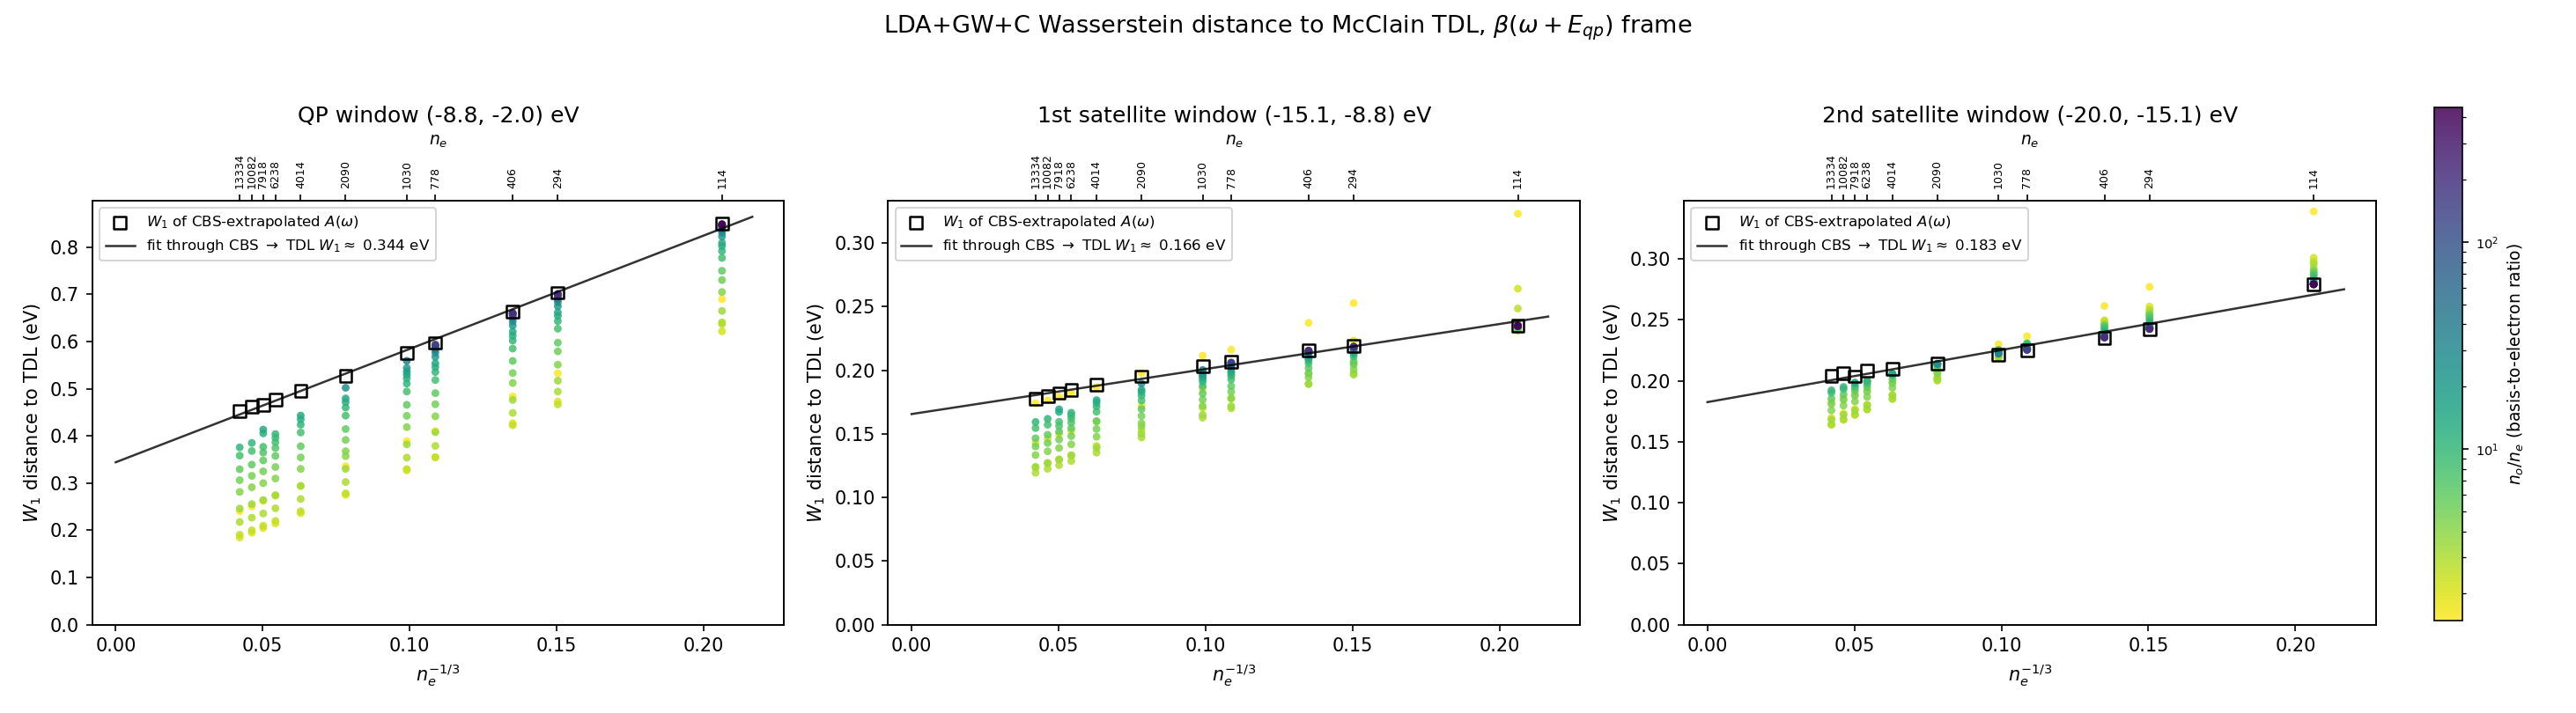
\includegraphics[width=\textwidth]{26/8/8-07/mcclain_gwc_wasserstein_eqp.png}
        % \caption{LDA+GW}
    \end{figure}
\end{frame}
\begin{frame}
    \frametitle{LDA+GW+C Loos' convention}
We are using 
\begin{equation}
    C_k^R(t) = \frac{1}{\pi}\int d\omega \frac{|\operatorname{Im} \Sigma^R_k(\omega+{\epsilon^{LDA}_k})|}{\omega^2} \left( e^{-i\omega t} + i\omega t - 1 \right).
\end{equation}
\pause
    \begin{figure}
        \centering
        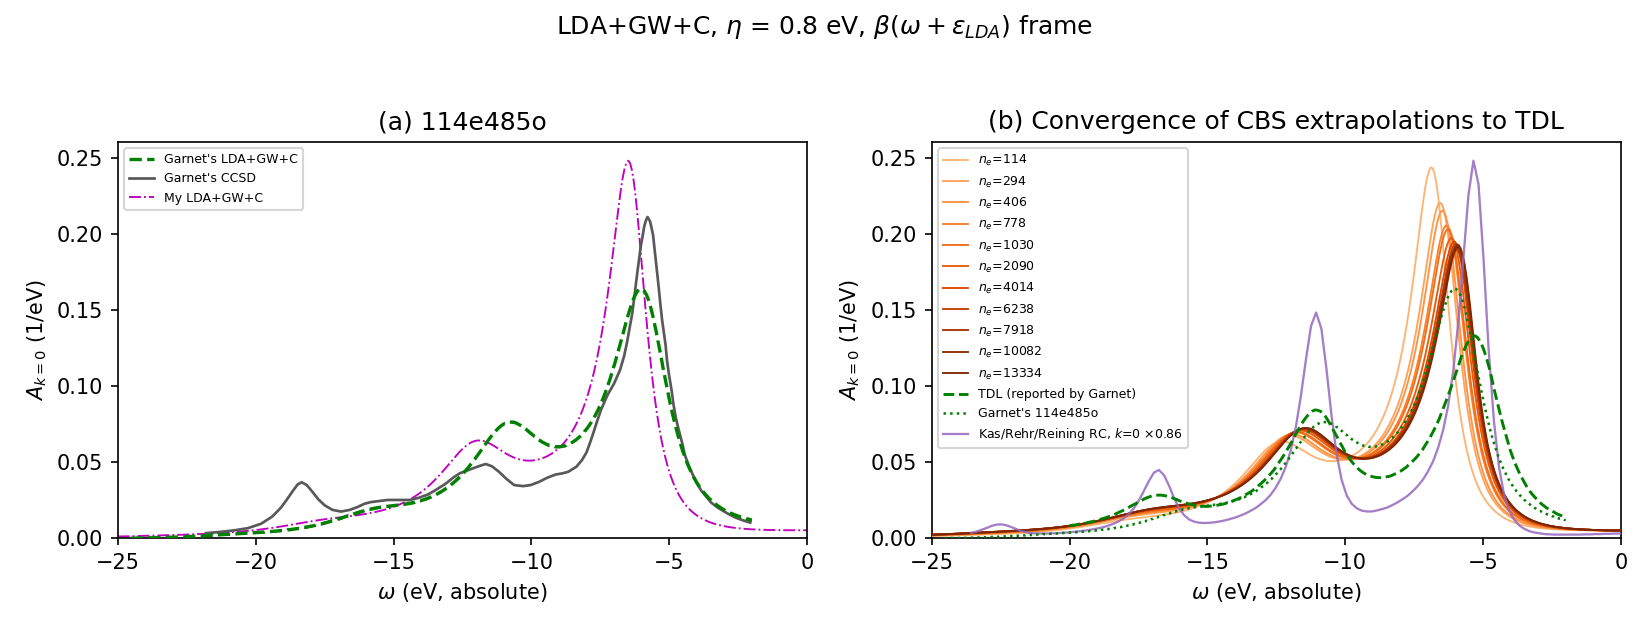
\includegraphics[width=\textwidth]{26/8/8-07/mcclain_gwc_compare.png}
        % \caption{LDA+GW}
    \end{figure}
\end{frame}
\begin{frame}
    \frametitle{LDA+GW+C Loos' convention continued}
    \begin{figure}
        \centering
        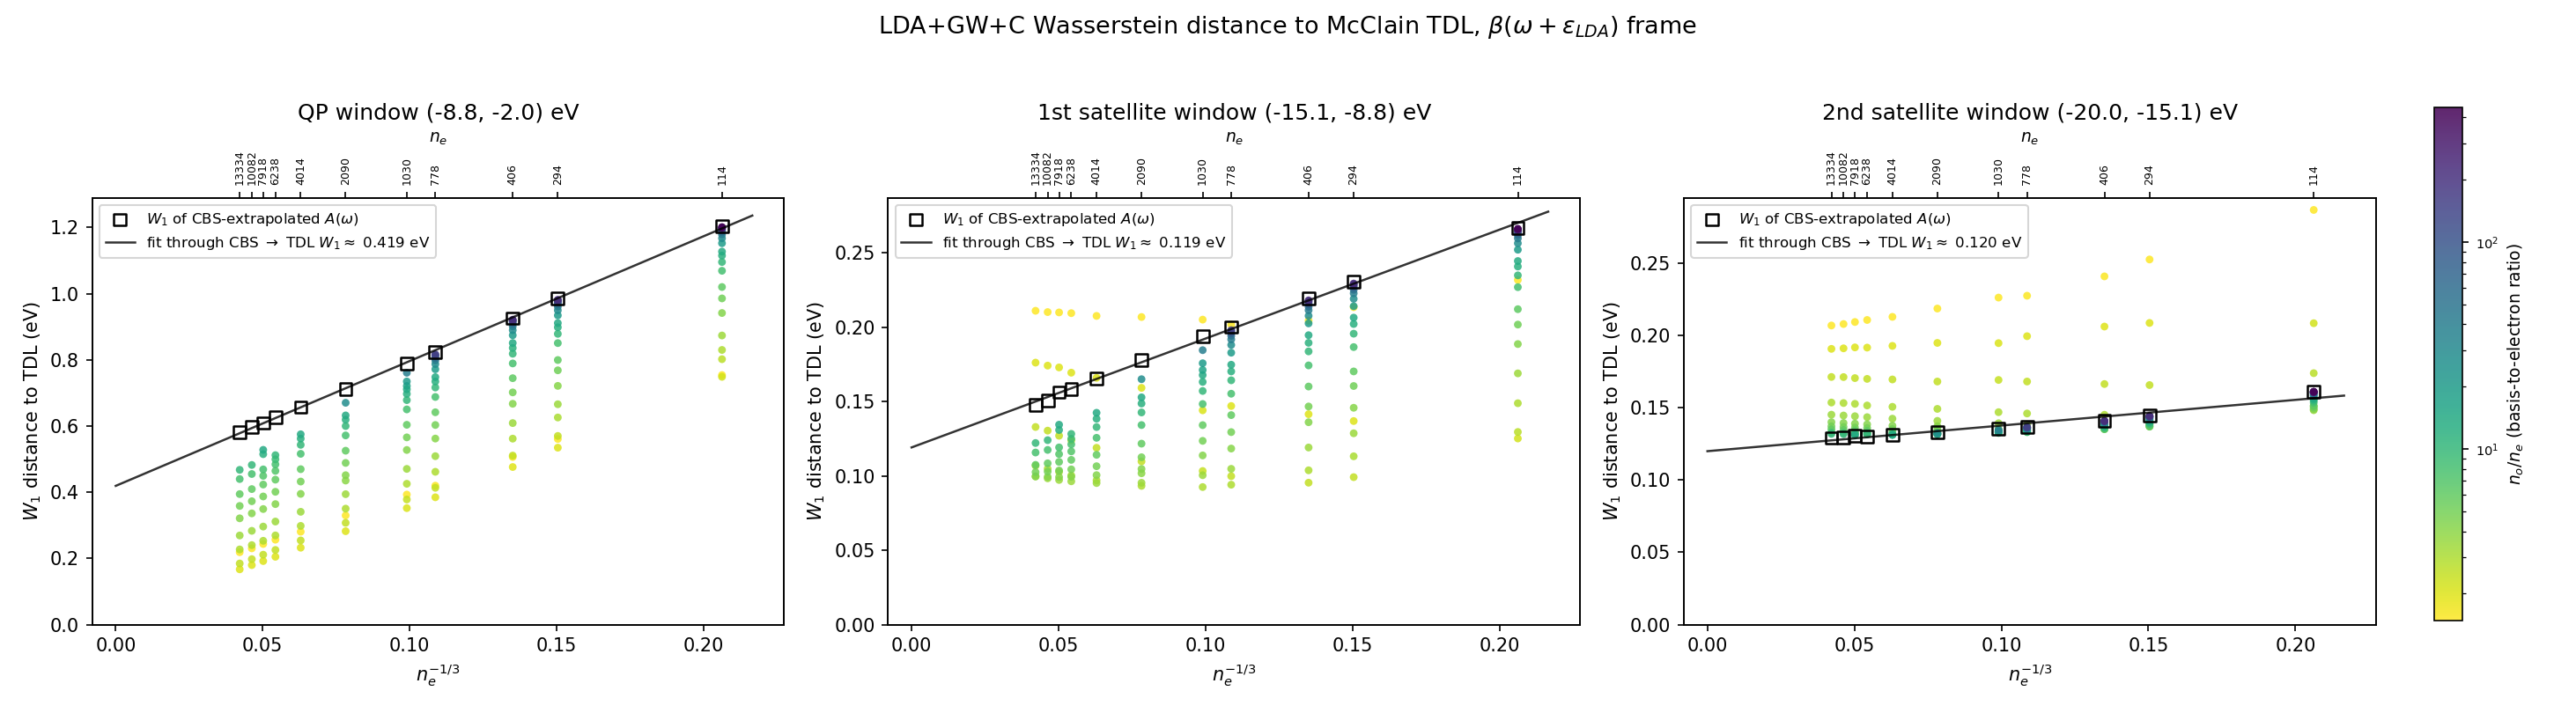
\includegraphics[width=\textwidth]{26/8/8-07/mcclain_gwc_wasserstein.png}
        % \caption{LDA+GW}
    \end{figure}
\end{frame}
\section{What to do next}
\begin{frame}
    \frametitle{What I have done so far}
\begin{enumerate}
\item Reproduced Garnet's LDA+GW curve for 14e19o and 114e485o \pause
    \begin{itemize}
        \item Wrote an LDA code for the UEG that we verified against PySCF \pause
        \item Wrote a GW code for the UEG that we verified against PySCF \pause
    \end{itemize}
\item Reproduced Loos' finite basis HF+GW+C curves for molecules \pause
    \begin{itemize}
        \item This was only for valence states and not using LDA reference \pause
    \end{itemize}
\item Told Claude Code about all the above and asked it to reproduce Garnet's finite basis LDA+GW+C, but nothing came close \pause   
\end{enumerate}
What should we do next?
\end{frame}

\section{Applying dCC to the UEG spectral function}
\begin{frame}
    \frametitle{How I think we could apply dCC ideas to the UEG spectral function}
Consider
\begin{equation}
H_p^{\rm eff}
=
\epsilon_p^{\rm MF} a_p^{\dagger} a_p
+
\sum_{m\nu}
\Delta_{pm\nu}
B_{pm\nu}^{\dagger}
B_{pm\nu}
+ a_p^{\dagger} a_p
\sum_{m\nu}
\left(
\mathcal{M}_{pm\nu}
B_{pm\nu}^{\dagger}
+
\mathcal{M}_{pm\nu}^{*}
B_{pm\nu}
\right),
\end{equation}
with QB operators $B_{pm\nu}^{\dagger}$. \pause
$\Delta_{pm\nu} = \epsilon_p^{\rm MF} - \epsilon_m^{\rm MF} + \operatorname{sgn}(\epsilon_m^{\rm MF} - \epsilon^{\rm MF}_{k_F})\Omega_\nu$ and $\mathcal{M}_{pm\nu}$ are QB excitation energies and couplings, respectively. \pause
This is used to obtain Green's functions for GW+C and PT2+C. \pause It seems to me that in order to get Hamlin's dCC, instead of getting bosonic quantites from the QBA, one gets them with DFPT.
\end{frame}

\section{Madelung treatment }
\begin{frame}
    \frametitle{Derivation from HF total energy}
\begin{align}
    \red{E_{\rm HF}}(N) &= \sum_{\mathbf k} \green{\frac{k^2}{2}}\, n_k + \green{E_x} - \frac{N\red{|v_M|}}{2} \label{eq:hf_energy_1} \\
    &= \sum_{\mathbf k} \left(\green{\frac{k^2}{2}} - \red{\frac{|v_M|}{2}}\right) n_k + \green{E_x} \label{eq:hf_energy_2}
\end{align}\pause
with $
    \green{\Sigma^x_k} = -\frac{1}{\Omega}\sum_{\mathbf{q}\neq0} v_q\, n_{\mathbf{k}+\mathbf{q}}$\pause and
$    \green{E_x} = -\frac{1}{2\Omega}\sum_{\mathbf{k}}\sum_{\mathbf{q}\neq0} v_q\, n_{\mathbf{k}} n_{\mathbf{k}+\mathbf{q}}
    = -\frac{1}{2\Omega}\sum_{\mathbf{k}\neq\mathbf{k}'} v_{\mathbf{k}-\mathbf{k}'}\, n_{\mathbf{k}} n_{\mathbf{k}'}
    = \frac{1}{2}\sum_{\mathbf{k}}\green{\Sigma^x_k}\, n_{\mathbf{k}}$.\pause Then,
\begin{align}
    \rm IP &\equiv \red{E_{\rm HF}}(N-1) - \red{E_{\rm HF}}(N), \quad     \rm EA \equiv \red{E_{\rm HF}}(N+1) - \red{E_{\rm HF}}(N)\\
    &= -\left(\green{\frac{i^2}{2}} + \green{\Sigma^x_i}\right) + \frac{\red{|v_M|}}{2}, \qquad =\left(\green{\frac{a^2}{2}} + \green{\Sigma^x_a}\right) - \frac{\red{|v_M|}}{2} 
    % &\equiv -\red{F^{\rm HF}_i},
\end{align} \pause
since $
    \green{E_x}(N-1)
    = \green{E_x}(N) - \green{\Sigma^x_i}$ and $
    \green{E_x}(N+1)
    = \green{E_x}(N) + \green{\Sigma^x_a}$.
\end{frame}
\begin{frame}
    \frametitle{Why this is the proper interpretation of your paper }
 I interpret what you write after equation 64 as saying that it makes no difference whether the Madelung constant gets lumped into the single-particle energies, as in Eq.~(\ref{eq:hf_energy_2}), or added afterwards as in Eq.~(\ref{eq:hf_energy_1}). \pause I interpret what you write after equation 66 as saying that 
\begin{align}
    E_g &\equiv EA + \frac{\red{|v_M|}}{2} + IP + \frac{\red{|v_M|}}{2}\\
    &= \left(\green{\frac{j^2}{2}} + \green{\Sigma^x_j} - \frac{\red{|v_M|}}{2}\right) + \left[-\left(\green{\frac{i^2}{2}} + \green{\Sigma^x_i}\right) + \frac{\red{|v_M|}}{2}\right]+ \red{|v_M|}\\
&= \green{\frac{j^2}{2}} + \green{\Sigma^x_j} - \green{\frac{i^2}{2}} - \green{\Sigma^x_i} + \red{|v_M|} \label{eq:band_gap_madelung}
\end{align}
\end{frame}
\begin{frame}
    \frametitle{Consistency with QCPBC convention}
Band gaps are consistent (equation~(\ref{eq:band_gap_madelung})). \pause Previously used shifted Ewald summation, where $v_q = \begin{cases} \frac{4\pi}{q^2}, & q\neq 0\\ -\Omega\red{v_M}, & q=0\end{cases}$\pause, so total energies were 
\begin{align}
    \red{E_{\rm HF}}(N) &= \sum_{\mathbf k} \green{\frac{k^2}{2}}\, n_k - \frac{1}{2}\sum_{\mathbf{k}} n_{\mathbf{k}}\left(\frac{1}{\Omega}\sum_{\mathbf{q}} v_q\, n_{\mathbf{k}+\mathbf{q}}\right) \\
    &= \sum_{\mathbf k} \green{\frac{k^2}{2}}\, n_k - \frac{1}{2}\sum_{\mathbf{k}} n_{\mathbf{k}}\left(\frac{1}{\Omega}\left[\sum_{\mathbf{q}\neq 0} v_q\, n_{\mathbf{k}+\mathbf{q}} + \Omega\red{|v_M|}\, n_{\mathbf{k}}\right]\right) \\
    &= \sum_{\mathbf k} \green{\frac{k^2}{2}}\, n_k + \frac{1}{2}\sum_{\mathbf{k}}\green{\Sigma^x_k}\, n_{\mathbf{k}} - \frac{\red{|v_M|}}{2}\sum_{\mathbf{k}} n_{\mathbf{k}}^2 \\
    &= \sum_{\mathbf k} \green{\frac{k^2}{2}}\, n_k + \green{E_x} - \frac{N\red{|v_M|}}{2}.
\end{align} \pause
Recall that HF energies came out to be $\varepsilon^{\rm HF}_k = \green{\frac{k^2}{2}} + \green{\Sigma^x_k} - \red{|v_M|}\, n_{\mathbf{k}}$.
\end{frame}
\begin{frame}
    \frametitle{How BW changes} Define $\green{E^{(0)}_{ij\to ab}} = \green{\varepsilon_a} + \green{\varepsilon_b} - \green{\varepsilon_i} - \green{\varepsilon_j}$. \pause 
Since $\operatorname{Tr}(\mathbf{W}^{O}) - \operatorname{Tr}(\mathbf{W}^{V})=E^{(2)}$, \pause
\textbf{Before} and \textbf{Now}, respectively:\begin{align}
\red{{E}^{(2)}} &= -\sum_{ijab}\frac{\green{\mathcal{K}_{ij}^{ab}}}{{\red{\tilde{E}_{ij\rightarrow ab}^{(0)}}}}\\
\red{\tilde{E}_{ij\rightarrow ab}^{(0)}}&= \green{E^{(0)}_{ij\to ab}}+2\red{|v_M|}\\
\Sigma^{(2)}_{pp}(\omega) &= \sum_{ija} \frac{\green{\mathcal{K}_{ij}^{ap}}}{\omega -\green{\epsilon^i} + \left( \green{\epsilon_a} - \green{\epsilon_j}\right) - 2\red{|v_M|}} + \sum_{iab} \frac{\green{\mathcal{K}_{ip}^{ab}}}{\omega-\green{\epsilon_a} - \left(\green{\epsilon_b} - \green{\epsilon_i}\right) + \red{|v_M|}} \end{align} \pause
\begin{align}
\green{E^{(2)}} &= -\sum_{ijab}\frac{\green{\mathcal{K}_{ij}^{ab}}}{{\green{E_{ij\rightarrow ab}^{(0)}}}}\\
\Sigma^{(2)}_{pp}(\omega)&= \sum_{ija} \frac{\green{\mathcal{K}_{ij}^{ap}}}{\omega-\green{\epsilon_i} + \left( \green{\epsilon_a} - \green{\epsilon_j}
\right)+ \frac{\red{|v_M|}}{2}} + \sum_{iab} \frac{\green{\mathcal{K}_{ip}^{ab}}}{\omega-\green{\epsilon_a} - \left(\green{\epsilon_b} - \green{\epsilon_i}\right)+ \frac{\red{|v_M|}}{2}}
\end{align}

\end{frame}
\begin{frame}
    \frametitle{Updated results: BW 4,0}
\begin{figure}
    \centering
    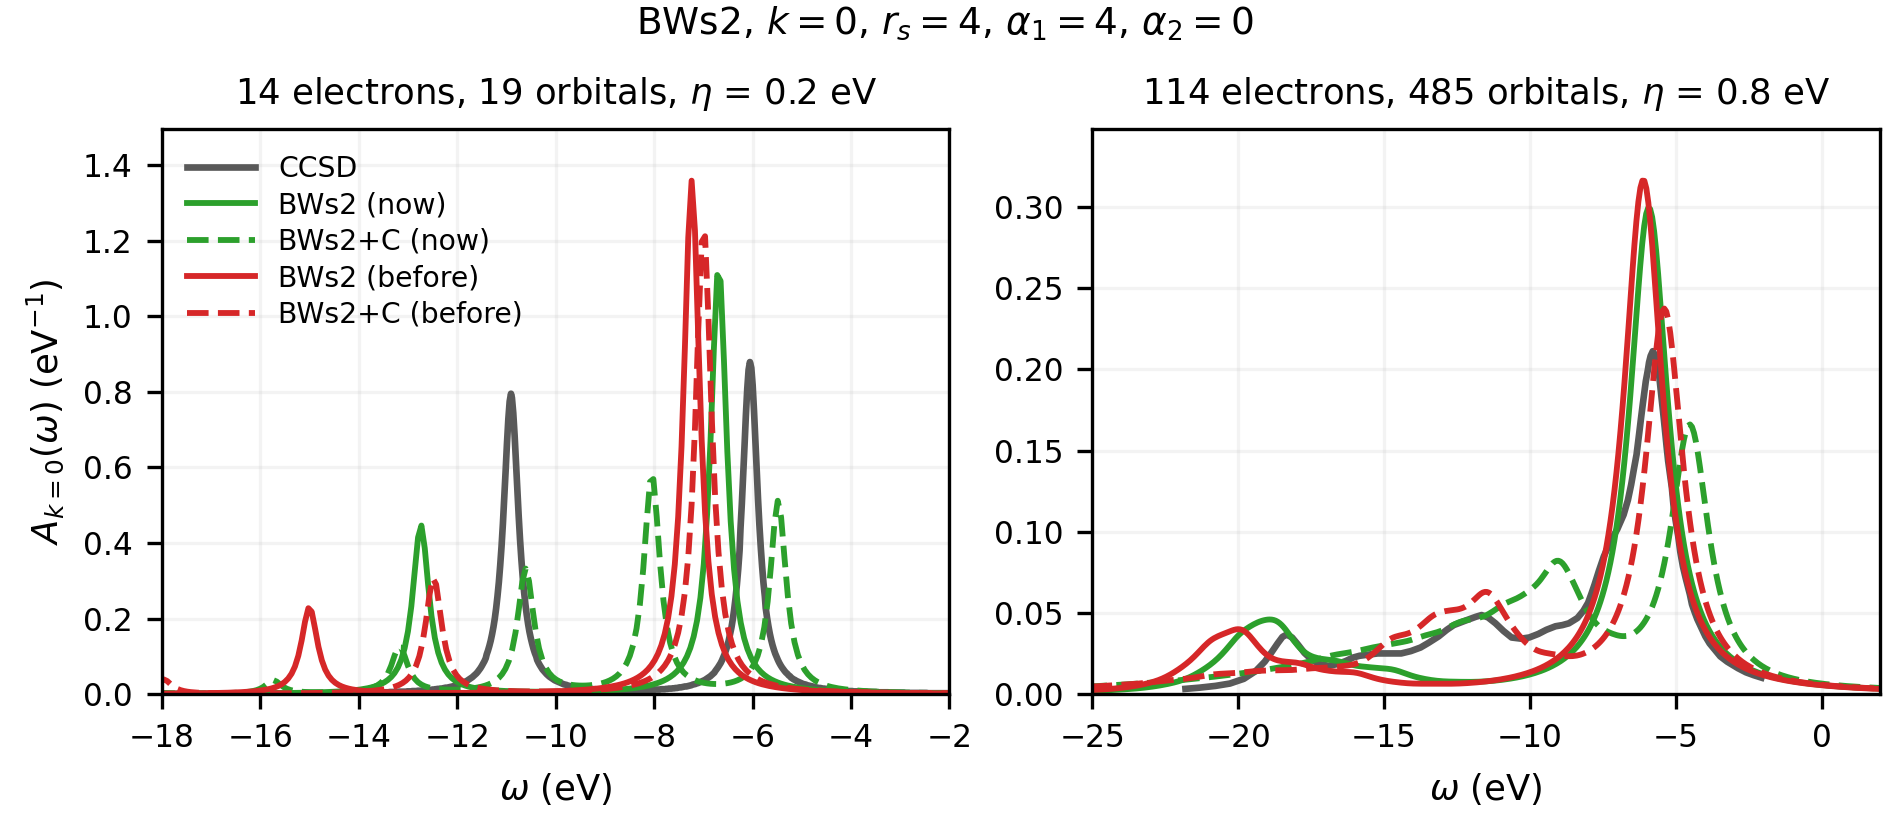
\includegraphics[width=\textwidth]{26/10/07/k0_twopanel_fig3_bws2_a40.png}
\end{figure}
\end{frame}
\begin{frame}
    \frametitle{Updated results: BW 2,2}
\begin{figure}
    \centering
    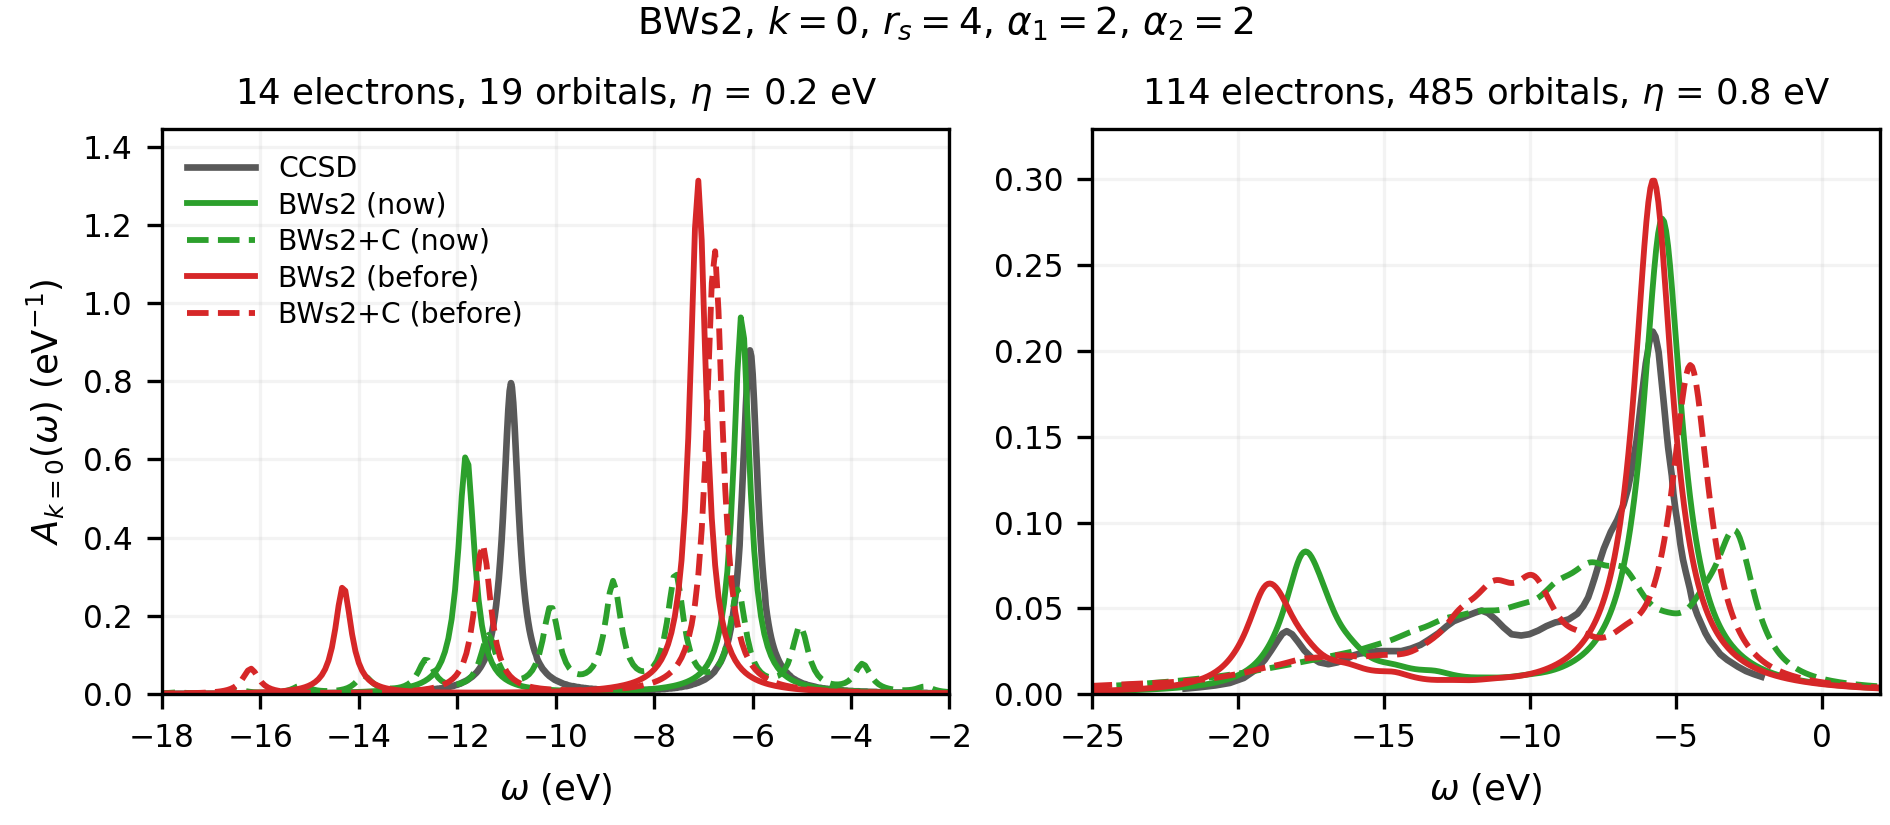
\includegraphics[width=\textwidth]{26/10/07/k0_twopanel_fig4_bws2_a22.png}
\end{figure}
\end{frame}
\begin{frame}
    \frametitle{How HF+GW changes}
1. Calculate the RPA polarizability   
\begin{align}
    &\left(\begin{array}{ll}
\mathrm{A} & \mathrm{~B} \\
\mathrm{~B} & \mathrm{~A}
\end{array}\right)\left(\begin{array}{ll}
\mathrm{X} & \mathrm{Y} \\
\mathrm{Y} & \mathrm{X}
\end{array}\right)=\left(\begin{array}{cc}
\mathrm{X} & -\mathrm{Y} \\
-\mathrm{Y} & \mathrm{X}
\end{array}\right)\left(\begin{array}{ll}
\Omega & 0 \\
0 & \Omega
\end{array}\right)\end{align} \pause
2. Form the correlation self-energy as
\begin{align}
\Sigma_{pp}^{c,G_0W_0}(\omega)&= \sum_{j \nu}\frac{W_{p j \nu} W_{p j \nu}}{\omega-\left(\epsilon_j-\Omega_\nu\right)-\mathrm{i} \eta} + \sum_{b \nu}\frac{W_{p b \nu} W_{p b \nu}}{\omega-\left(\epsilon_b+\Omega_\nu\right)+\mathrm{i} \eta},
\end{align}
where $W_{n p \nu}=\sqrt{2}\sum_{i a} V_{n p i a}(\mathbf{X}+\mathbf{Y})_{i a, \nu}$ with $V_{n p i a}=(n i|p a)$.
\end{frame}
\begin{frame}
    \frametitle{How HF+GW changes cont.}
\textbf{Before }:
\begin{align*}
    A_{ia,jb} &= \delta_{ij}\delta_{ab}\left(\green{\epsilon_a}-\green{\epsilon_i}+\red{|v_M|}\right)+\langle\Phi_i^a|\green{\hat V_{\rm res}}|\Phi_j^b\rangle\\
    &= \delta_{ij}\delta_{ab}\left(\green{\epsilon_a}-\green{\epsilon_i}\right)+\langle\Phi_i^a|\green{\hat V_{\rm res}}|\Phi_j^b\rangle\\
B_{ia,jb} &= \langle\Phi_i^a|\green{\hat V_{\rm res}}|\Phi_j^b\rangle \\
    \Sigma_{pp}^{c,G_0W_0}(\omega)&= \sum_{j \nu}\frac{\red{W_{p j \nu}} \red{W_{p j \nu}}}{\omega-\left(\green{\epsilon_j}-\red{|v_M|}-\red{\Omega_\nu}\right)+\mathrm{i} \eta} + \sum_{b \nu}\frac{\red{W_{p b \nu}} \red{W_{p b \nu}}}{\omega-\left(\green{\epsilon_b}+\red{\Omega_\nu}\right)+\mathrm{i} \eta}
\end{align*}
\pause 
\textbf{Now }: 
\begin{align}
    A_{ia,jb} &= \delta_{ij}\delta_{ab}\left(\green{\epsilon_a}-\red{\frac{|v_M|}{2}}-\green{\epsilon_i}+\red{\frac{|v_M|}{2}}\right)+\langle\Phi_i^a|\green{\hat V_{\rm res}}|\Phi_j^b\rangle\\
    &= \delta_{ij}\delta_{ab}\left(\green{\epsilon_a}-\green{\epsilon_i}\right)+\langle\Phi_i^a|\green{\hat V_{\rm res}}|\Phi_j^b\rangle\\
B_{ia,jb} &= \langle\Phi_i^a|\green{\hat V_{\rm res}}|\Phi_j^b\rangle \\
    \Sigma_{pp}^{c,G_0W_0}(\omega)&= \sum_{j \nu}\frac{\green{W_{p j \nu}} \green{W_{p j \nu}}}{\omega-\left(\green{\epsilon_j}+\red{\frac{v_M}{2}}-\green{\Omega_\nu}\right)+\mathrm{i} \eta} + \sum_{b \nu}\frac{\green{W_{p b \nu}} \green{W_{p b \nu}}}{\omega-\left(\green{\epsilon_b}+\red{\frac{v_M}{2}}+\green{\Omega_\nu}\right)+\mathrm{i} \eta}
\end{align}
\end{frame}
\begin{frame}
    \frametitle{Updated results: HF+GW}
\begin{figure}
    \centering
    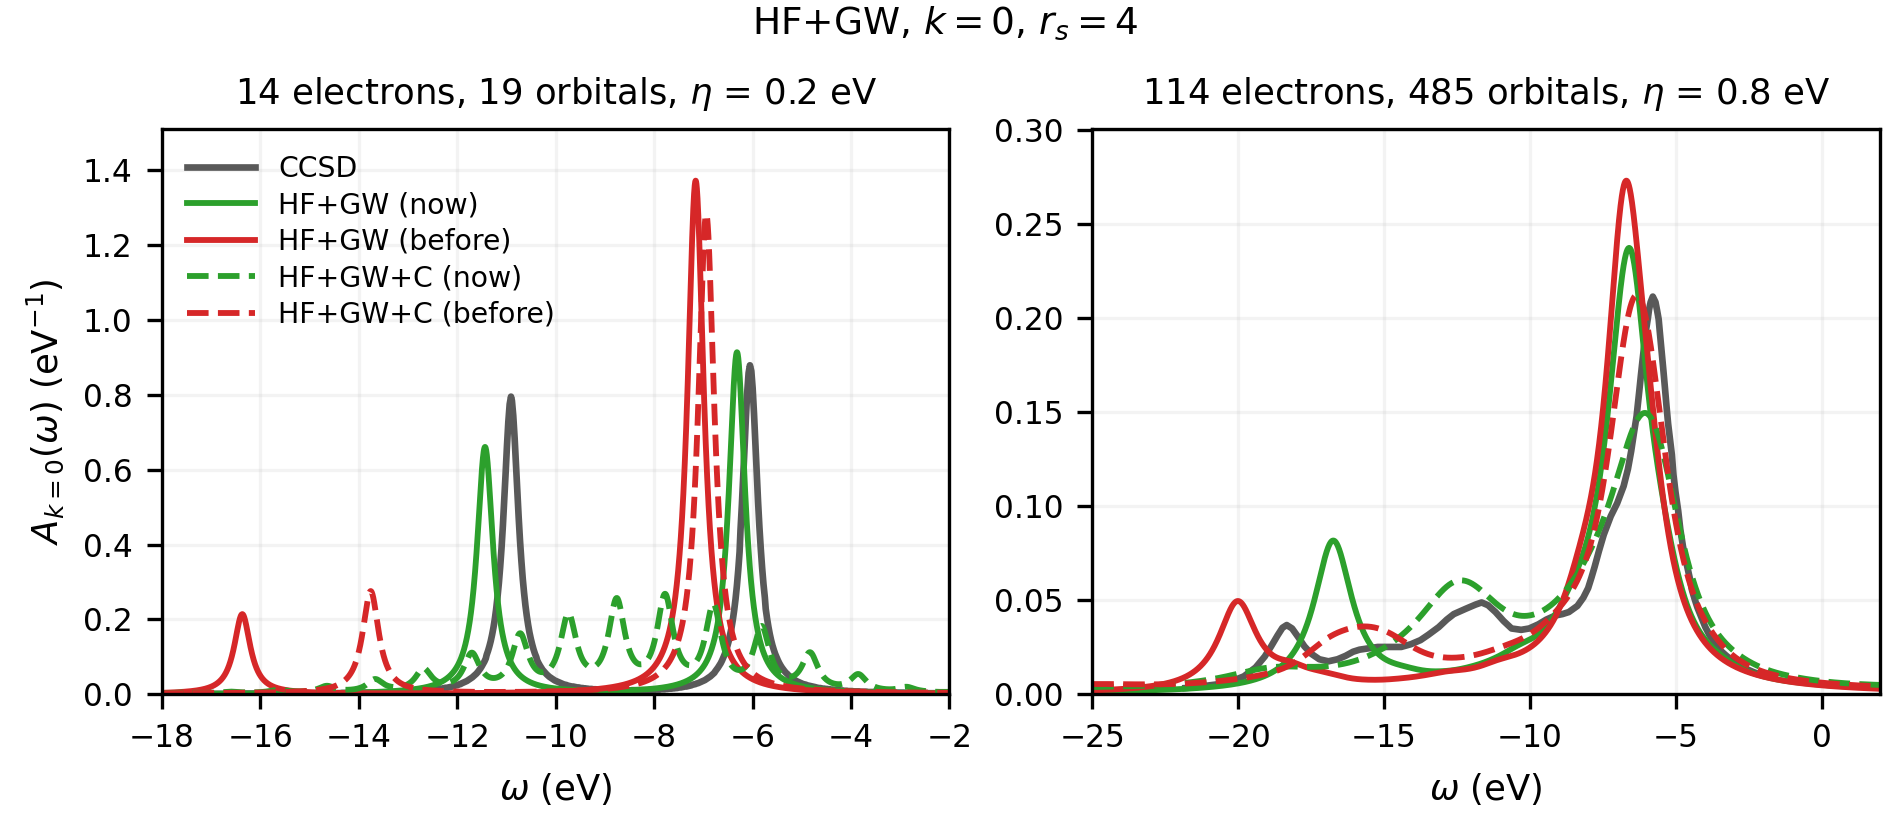
\includegraphics[width=\textwidth]{26/10/07/k0_twopanel_fig1a_hfgw_now_vs_before.png}
\end{figure}
\end{frame}
\begin{frame}
    \frametitle{Comparing updated HF+GW to LDA+GW}
\begin{figure}
    \centering
    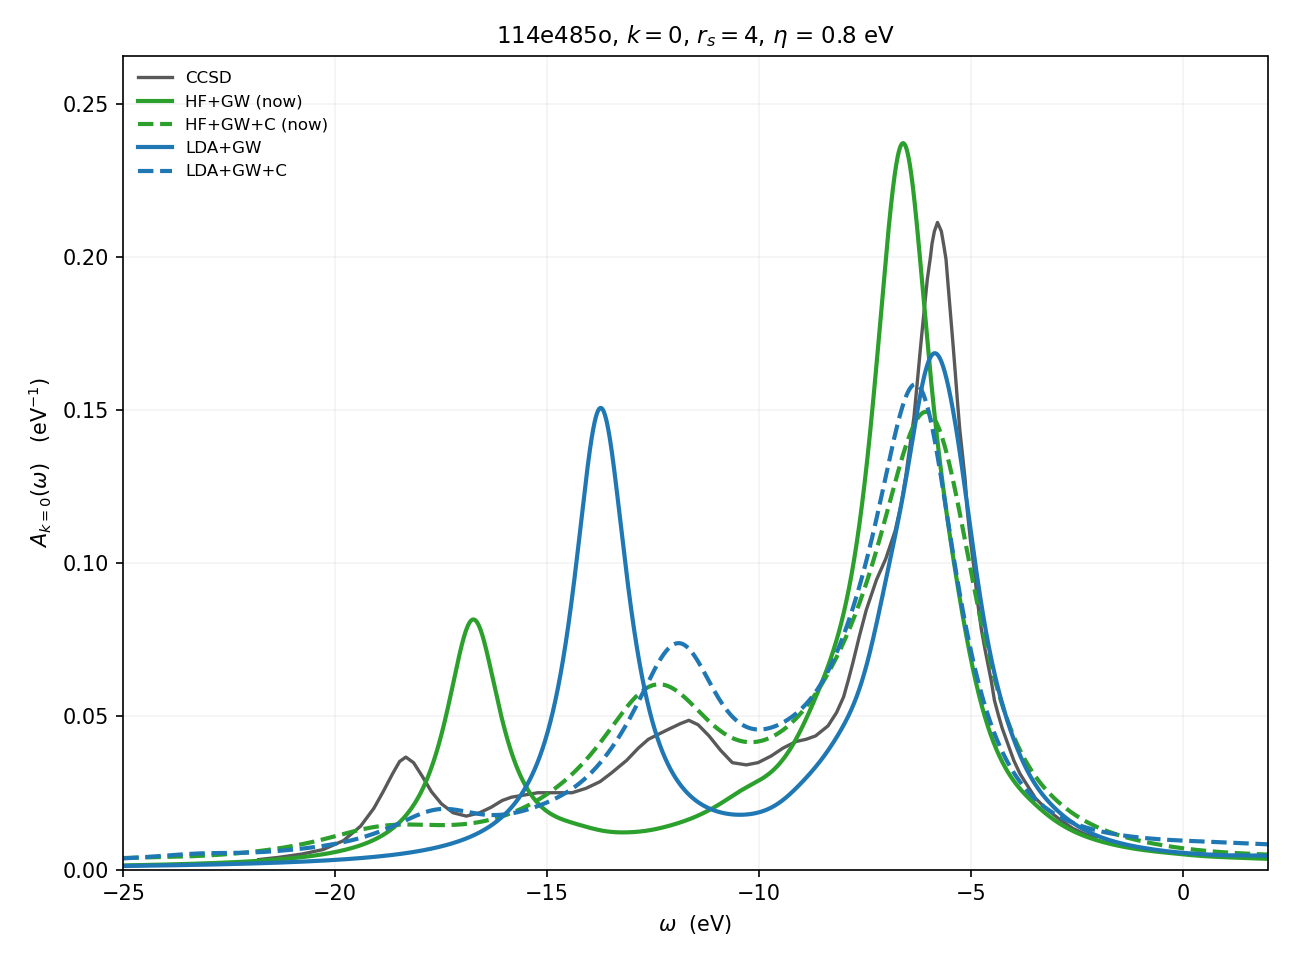
\includegraphics[width=0.9\textwidth]{26/10/07/k0_114e485o_fig1b_hfgw_now_vs_lda.png}
\end{figure}
\end{frame}
\begin{frame}
    \frametitle{Things to do now}
\begin{enumerate}
    \item Rerun Holm style SCCE(GW0) with Madelung correction. \pause
    \item Rerun CCSD with Madelung correction. \pause
\item Redo all TDL extrapolations with Madelung correction.
    \end{enumerate}
\end{frame}
\section{Derivation of the quasiboson Hamiltonian }
\begin{frame}
    \frametitle{The goal}
With $\epsilon_{\mathbf k}^{(0)}=\frac{k^2}{2}+\frac{v_M}{2}$ and $v_M=-2.837297 \times\left(\frac{3}{4 \pi}\right)^{1 / 3} N^{-1 / 3} r_s^{-1}$
\begin{align}
\hat H
&=
\sum_{\mathbf k}\epsilon_{\mathbf k}^{(0)}\hat a_{\mathbf k}^\dagger \hat a_{\mathbf k}
+
{\frac{1}{2\Omega}
\sum_{\mathbf q\neq\mathbf 0}v_q
\sum_{\mathbf k\mathbf k'}
a_{\mathbf{k}+\mathbf q}^\dagger
a_{\mathbf{k}'-\mathbf q}^\dagger
a_{\mathbf k'}
a_{\mathbf k}}\\
&=
E_{\rm HF}
+
{\sum_{\mathbf k}
\epsilon_{\mathbf k}^{\rm HF}
:
\hat a_{\mathbf k}^\dagger \hat a_{\mathbf k}
:}
+
\frac{1}{2\Omega}
\sum_{\mathbf q\neq\mathbf 0}v_q
\sum_{\mathbf k\mathbf k'}:
a_{\mathbf{k}+\mathbf q}^\dagger
a_{\mathbf{k}'-\mathbf q}^\dagger
a_{\mathbf k'}
a_{\mathbf k}:
\end{align}
where ${
\epsilon_{\mathbf k}^{\rm HF}
}
=
\frac{k^2}{2}
+
\frac{v_M}{2}
-
\frac{1}{\Omega}
\sum_{\mathbf q\neq\mathbf 0}
v_q n_{\mathbf{k}+\mathbf q}
$. \pause We want to get to 
\begin{equation}
    \hat H_{\rm eb}
    =
    -\sum_{\mathbf k\in\mathcal O}
    \epsilon_{\mathbf k}^{\rm HF}
    h_{\mathbf k}^{\dagger}h_{\mathbf k}
    +
    \sum_{\nu_{\mathbf q}}
    \omega_{\nu_{\mathbf q}}^{\rm pl}
    \hat\beta_{\nu_{\mathbf q}}^{\dagger}
    \hat\beta_{\nu_{\mathbf q}}
    +
    \sum_{\mathbf k\mathbf q}
    \sum_{\nu_{\mathbf q}}
    g_{\nu}^{\rm pl}(\mathbf k,\mathbf q)
    h_{\mathbf k+\mathbf q}^{\dagger}
    h_{\mathbf k}
    \left(
        \hat\beta_{\nu_{\mathbf q}}
        +
        \hat\beta_{\nu_{-\mathbf q}}^{\dagger}
    \right).
\end{equation}
\end{frame}
\begin{frame}
    \frametitle{Quadratic bosonic bath}
Define  $
    E_{i\mathbf q}^{\dagger}
    =
    a_{\mathbf{i}+\mathbf q}^{\dagger}a_{\mathbf i}$ and $
    E_{i\mathbf -q}
    =
    a_{\mathbf i}^{\dagger}a_{\mathbf{i}-\mathbf q}$ with $\hat\kappa[\mathbf z]
    =
    \sum_{i\mathbf q}
    \left[
        \kappa_{i\mathbf q}
        E_{i\mathbf q}^{\dagger}
        -
        \kappa_{i\mathbf q}^{*}
        E_{i\mathbf q}
    \right]$ using $
    \boldsymbol{\kappa}_{\mathbf q}
    =
    \begin{pmatrix}
        \kappa_{1\mathbf q}\\
        \kappa_{2\mathbf q}\\
        \vdots
    \end{pmatrix}
$ and $
    {
    \mathbf z_{\mathbf q}
    =
    \begin{pmatrix}
        \boldsymbol{\kappa}_{\mathbf q}\\
        \boldsymbol{\kappa}_{-\mathbf q}^{*}
    \end{pmatrix}
    }
$. \pause Given $    |\Phi(\mathbf z)\rangle
    =
    e^{\hat\kappa[\mathbf z]}
    |\Phi_0\rangle$, we have \begin{align}
    E(\mathbf z)
    &=
    \langle\Phi(\mathbf z)|
    \hat H
    |\Phi(\mathbf z)\rangle
    \\
    % &=
    % \langle\Phi_0|
    % e^{-\hat\kappa[\mathbf z]}
    % \hat H
    % e^{\hat\kappa[\mathbf z]}
    % |\Phi_0\rangle\\
    &=
    E_{\rm HF}
    +
    \langle\Phi_0|
    [\hat H,\hat\kappa[\mathbf z]]
    |\Phi_0\rangle
+
    \frac{1}{2}
    \langle\Phi_0|
    [[\hat H,\hat\kappa[\mathbf z]],\hat\kappa[\mathbf z]]
    |\Phi_0\rangle
    +
    \ldots \\ 
\implies     \nabla_{\mathbf z}E(\mathbf z)
    &=
    \begin{pmatrix}
        \dfrac{\partial E(\mathbf z)}
        {\partial\boldsymbol{\kappa}}\\
        \\
        \dfrac{\partial E(\mathbf z)}
        {\partial\boldsymbol{\kappa}^{*}}
    \end{pmatrix} \implies    \left.
    \nabla_{\mathbf z}E(\mathbf z)
    \right|_{\mathbf z=0}
    =
    0
    \label{eq:energy_expansion_kappa}
\end{align}
\end{frame}
\begin{frame}
    \frametitle{Quadratic bosonic bath cont.}
\begin{align}
    \mathcal H_{\rm HF}
    =
    \left.
    \frac{\partial^2 E(\mathbf z)}
    {\partial
    \begin{pmatrix}
        \boldsymbol{\kappa}^{*}\\
        \boldsymbol{\kappa}
    \end{pmatrix}
    \partial
    \begin{pmatrix}
        \boldsymbol{\kappa}&
        \boldsymbol{\kappa}^{*}
    \end{pmatrix}}
    \right|_{\mathbf z=0}
    &={
    \begin{pmatrix}
        A & B\\
        B^{*} & A^{*}
    \end{pmatrix}.
    }
\end{align} \pause
Thus, the second-order correction to the HF energy is
\begin{align}
E^{(2)}(\mathbf \kappa, \mathbf \kappa^{*})
    &=
    \frac{1}{2}
    \begin{pmatrix}
        \boldsymbol{\kappa}_{\mathbf q}^{*} &
        \boldsymbol{\kappa}_{-\mathbf q}
    \end{pmatrix}
    \begin{pmatrix}
        A & B\\
        B^{*} & A^{*}
    \end{pmatrix}
    \begin{pmatrix}
        \boldsymbol{\kappa}_{\mathbf q}\\
        \boldsymbol{\kappa}_{-\mathbf q}^{*}
    \end{pmatrix}
\end{align}\pause
Quantizing the space and then applying Bogoliubov transformation gives 
\begin{align}
    \hat{H}^{(2)}&= \frac{1}{2}
    \begin{pmatrix}
        \hat{\bm{b}}_{\mathbf q}^{\dagger} &
        \hat{\bm{b}}_{-\mathbf q}
    \end{pmatrix}
    \begin{pmatrix}
        A & B\\
        B^{*} & A^{*}
    \end{pmatrix}
    \begin{pmatrix}
        \hat{\bm{b}}_{\mathbf q}\\
        \hat{\bm{b}}_{-\mathbf q}^{\dagger}
    \end{pmatrix}\\
    &=
    \hat{\bm{\beta}}_{\mathbf q}^{\dagger} \boldsymbol{\Omega}_{\mathbf q} \hat{\bm{\beta}}_{\mathbf q}
    +
    \frac{1}{2}\operatorname{Tr}(\boldsymbol{\Omega}_{\mathbf q}-A)+\frac{1}{2}\operatorname{Tr}(A)\\
&= \sum_{\nu_{\mathbf q}} \omega_{\nu_{\mathbf q}} \hat{\beta}_{\nu_{\mathbf q}}^{\dagger} \hat{\beta}_{\nu_{\mathbf q}} + E_{\rm RPA} + \frac{1}{2}\operatorname{Tr}(A)
\end{align}
\end{frame}
\begin{frame}
    \frametitle{Pure fermionic and coupling terms}
Start with 
\begin{equation}
    \hat H_{\rm h}(\boldsymbol{\kappa})
    =
    \sum_{\mathbf k,\mathbf k'\in\mathcal O}
    h^{\rm h}_{\mathbf k'\mathbf k}(\boldsymbol{\kappa})
    h_{\mathbf k'}^\dagger h_{\mathbf k}.
    \label{eq:hole_hamiltonian_kappa}
\end{equation} \pause Expand to first order about the
Hartree--Fock reference
\begin{align}
    h^{\rm h}_{\mathbf k'\mathbf k}(\boldsymbol{\kappa})
    &=
    h^{\rm h}_{\mathbf k'\mathbf k}(0)+
    \sum_{i\mathbf q}
    \left.
    \frac{\partial
    h^{\rm h}_{\mathbf k'\mathbf k}}
    {\partial\kappa_{i\mathbf q}}
    \right|_{0}
    \kappa_{i\mathbf q}+
    \sum_{i\mathbf q}
    \left.
    \frac{\partial
    h^{\rm h}_{\mathbf k'\mathbf k}}
    {\partial\kappa_{i\mathbf q}^{*}}
    \right|_{0}
    \kappa_{i\mathbf q}^{*}
    +
    \mathcal O(\kappa^2),
    \label{eq:hole_hamiltonian_expansion}
\end{align} 
\pause
\begin{align}
    \left.
    \frac{\partial
    h^{\rm h}_{\mathbf k+\mathbf q,\mathbf k}}
    {\partial\kappa_{i\mathbf q}}
    \right|_0
    &=
    -
    \left.
    \frac{\partial
    F_{\mathbf k,\mathbf k+\mathbf q}}
    {\partial\kappa_{i\mathbf q}}
    \right|_0
    \\
    &=
    -
    \sum_{\mathbf l}
    \frac{\partial
    F_{\mathbf k,\mathbf k+\mathbf q}}
    {\partial P_{\mathbf l + \mathbf q,\mathbf l}}
    \left.
    \frac{\partial
    P_{\mathbf l + \mathbf q,\mathbf l}}
    {\partial\kappa_{i\mathbf q}}
    \right|_0 \\
&= 
    -
\frac{v(\mathbf q)}{\Omega} \sum_{\mathbf l}
    \delta_{\mathbf l,\mathbf i}
\end{align}
\end{frame}
\begin{frame}
    \frametitle{Pure fermionic and coupling terms cont.}
So up to linear order in $\boldsymbol{\kappa}$
\begin{align}
    \hat H_{\rm h}(\boldsymbol{\kappa})
    &\overset{\text{direct}}{=} -
    \sum_{\mathbf k\in\mathcal O}
    \epsilon_{\mathbf k}^{\rm HF}
    h_{\mathbf k}^{\dagger}h_{\mathbf k}
-
    \sum_{\mathbf k\mathbf q}
    \sum_i
    \frac{v(\mathbf q)}{\Omega}
    h_{\mathbf k+\mathbf q}^{\dagger}h_{\mathbf k}
    \left(
        \kappa_{i\mathbf q}
        +
        \kappa_{i,-\mathbf q}^{*}
    \right)
    \label{eq:hole_hamiltonian_linear_kappa}
\end{align} \pause
Quantizing again and then applying the Bogoliubov transformation gives
\begin{align}
    \hat H_{\rm h-pl}
    &=
    \sum_{\mathbf k\mathbf q}
    \sum_{\nu_{\mathbf q}}
    g_{\nu}^{\rm pl}(\mathbf k,\mathbf q)
    h_{\mathbf k+\mathbf q}^{\dagger}
    h_{\mathbf k}
    \left(
        \hat\beta_{\nu_{\mathbf q}}
        +
        \hat\beta_{\nu_{-\mathbf q}}^{\dagger}
    \right),
    \label{eq:hole_plasmon_coupling}
\end{align} \pause
with
\begin{equation}
    {
    g_{\nu}^{\rm pl}(\mathbf k,\mathbf q)
    =
    -\frac{v(\mathbf q)}{\Omega}
    \sum_{\mathbf i}
    \left[
        X_{i\nu}(\mathbf q)
        +
        Y_{i\nu}(\mathbf q)
    \right].
    }
    \label{eq:screened_hole_plasmon_coupling}
\end{equation}\pause
So overall (omitting constant terms)
\begin{equation}
    \hat H_{\rm eb}
    =
    -\sum_{\mathbf k\in\mathcal O}
    \epsilon_{\mathbf k}^{\rm HF}
    h_{\mathbf k}^{\dagger}h_{\mathbf k}
    +
    \sum_{\nu_{\mathbf q}}
    \omega_{\nu_{\mathbf q}}^{\rm pl}
    \hat\beta_{\nu_{\mathbf q}}^{\dagger}
    \hat\beta_{\nu_{\mathbf q}}
    +
    \sum_{\mathbf k\mathbf q}
    \sum_{\nu_{\mathbf q}}
    g_{\nu}^{\rm pl}(\mathbf k,\mathbf q)
    h_{\mathbf k+\mathbf q}^{\dagger}
    h_{\mathbf k}
    \left(
        \hat\beta_{\nu_{\mathbf q}}
        +
        \hat\beta_{\nu_{-\mathbf q}}^{\dagger}
    \right).
\end{equation}


\end{frame}
\begin{frame}
    \frametitle{Results}
\begin{figure}
    \centering
    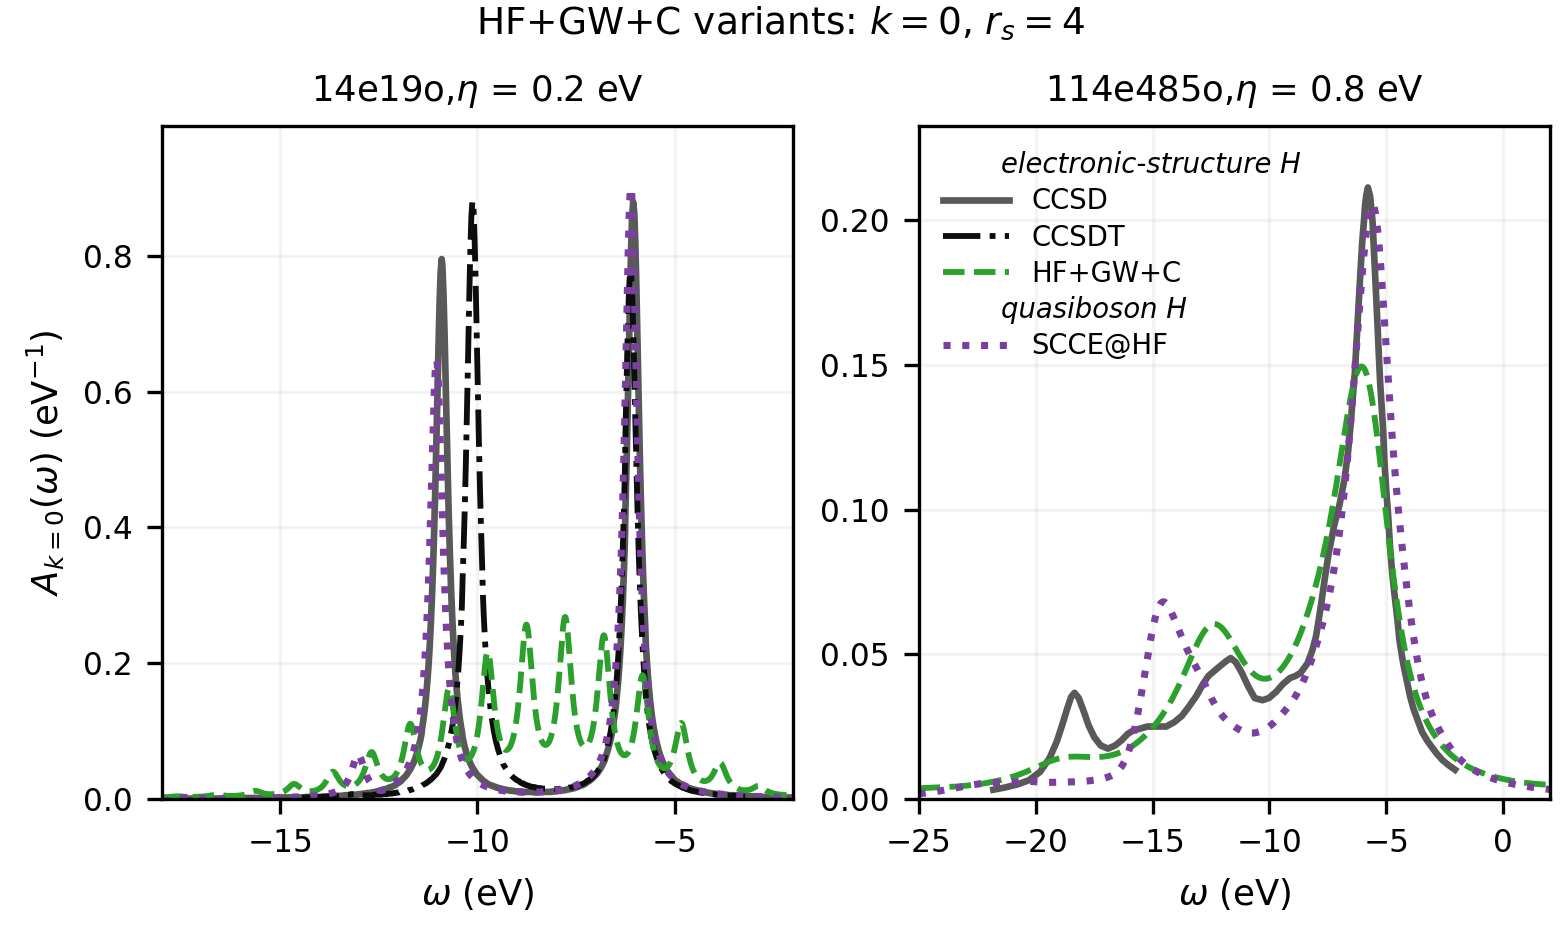
\includegraphics[width=\textwidth]{26/10/07/k0_twopanel_fig5_es_vs_qb.png}
\end{figure}
\end{frame}
\begin{frame}
    \frametitle{Results}
\begin{figure}
    \centering
    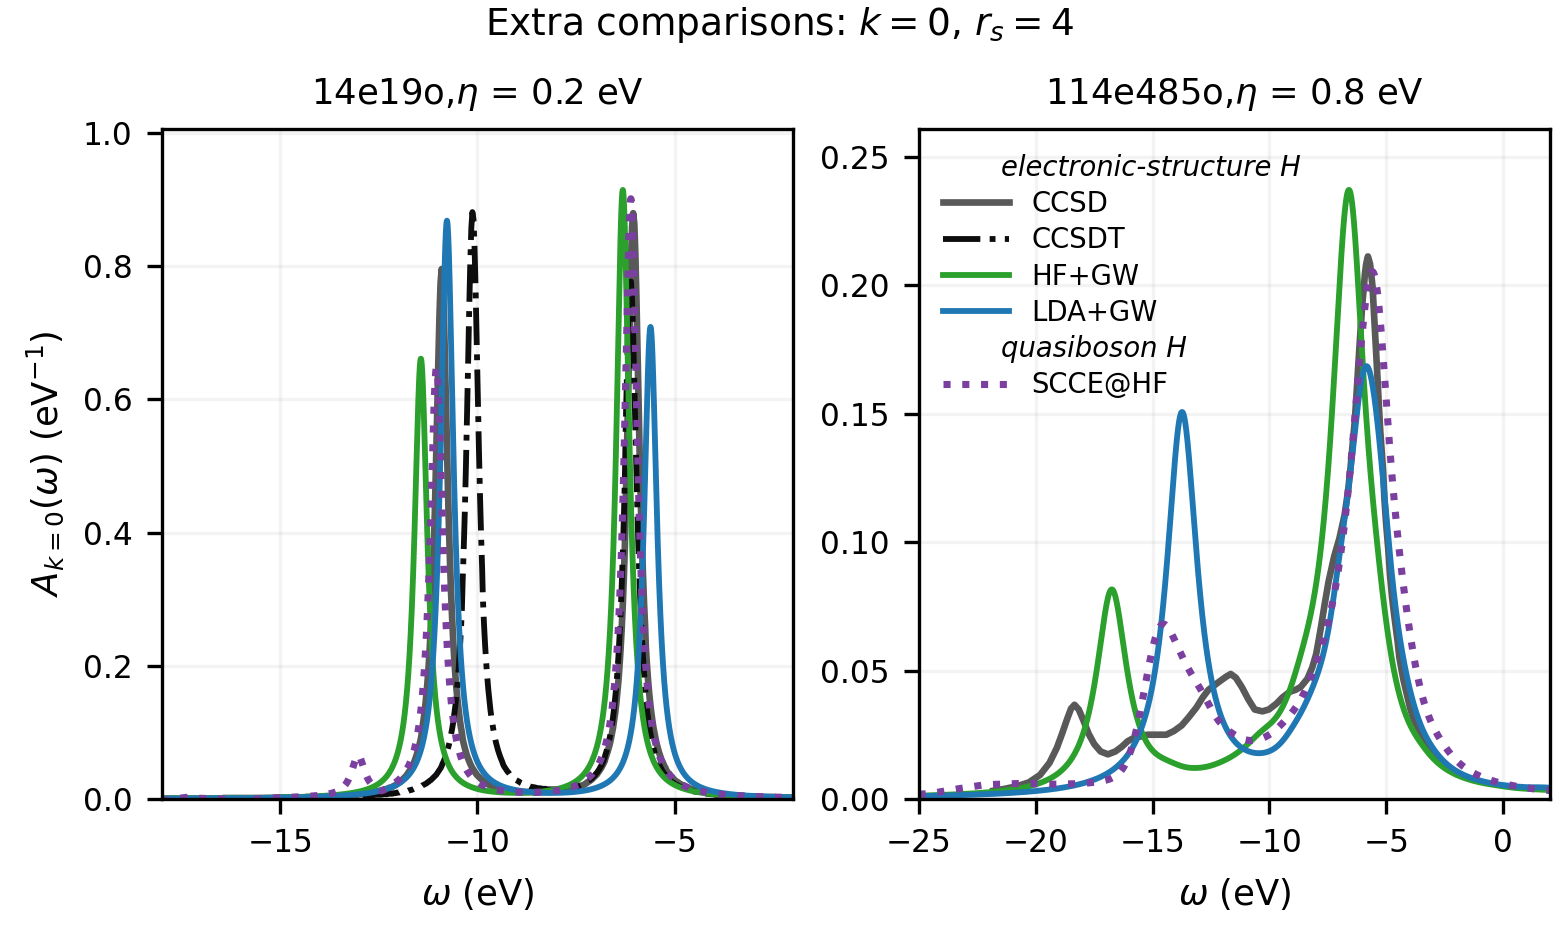
\includegraphics[width=\textwidth]{26/10/07/k0_twopanel_fig6_gw_frames_vs_scce.png}
\end{figure}
\end{frame}
\end{document}